\documentclass{article}

% Use [preprint] for unlimited pages (target: 12 main + 1 refs + appendix).
% Switch to plain \usepackage{neurips_2024} for the strict 9-page submission style.
\usepackage[preprint]{neurips_2024}

\usepackage[utf8]{inputenc}
\usepackage[T1]{fontenc}
\usepackage{hyperref}
\usepackage{url}
\usepackage{booktabs}
\usepackage{amsfonts}
\usepackage{amsmath}
\usepackage{amssymb}
\usepackage{mathtools}
\usepackage{nicefrac}
\usepackage{microtype}
\usepackage{xcolor}
\usepackage{graphicx}
\usepackage{subcaption}
\usepackage[capitalise,noabbrev]{cleveref}

\graphicspath{{../figures/}{../results/}{../}}

\title{Architecture- and Metric-Corrected Double Descent:\\
A Fractional-Width ResNet Recovers the Belkin--Nakkiran Curve}

\author{%
  Zhengda Li \\ \texttt{zl3651} \And
  Yusheng Li \\ \texttt{yl6009} \And
  Shufeng Chen \\ \texttt{sc5739} \And
  Yizheng Lin \\ \texttt{yl6079} \\
  \AND
  Department of Electrical Engineering, Columbia University\\
  EECS 6699: Mathematics of Deep Learning, Spring 2026
}

\begin{document}

\maketitle

\begin{abstract}
Double descent (DD) predicts that test risk peaks at the interpolation threshold and falls again in the over-parameterised regime. We reproduce textbook DD on random Fourier features (RFF) for MNIST, mechanistically attribute the peak to feature-Gram conditioning collapse via ridge and noise sweeps, and confirm a bias--variance decomposition with variance dominating the peak. The textbook neural-network DD curve is harder to surface: a naive CNN/ResNet width sweep on $n=4{,}000$ noisy CIFAR-10 fails because raw parameter count overshoots the effective interpolation threshold. We repair the capacity axis with a \emph{fractional-$k$} ResNet whose stage widths scale continuously through the threshold; on this family DD reappears as a clean rise--peak--valley--recovery curve, with test accuracy moving $26\%\!\to\!49\%\!\to\!53\%$ across $k\in[0.125,2]$ at $15\%$ label noise. Five independent diagnostics --- penultimate-feature stable rank, full empirical NTK, Bartlett (2020) effective rank, sample-wise peak migration, and Hessian top eigenvalue --- localise the same phase transition near $k\approx0.1875$. Finally we audit the evaluation protocol: reporting the best-over-epochs test accuracy systematically shallows the over-parameterised valley relative to final-epoch reporting, with the bias concentrated in exactly the regime where DD claims most depend on it.
\end{abstract}

\section{Introduction}
\label{sec:intro}

Classical statistical learning theory predicts a single U-shaped relationship between model capacity and test risk: increasing $p$ first reduces bias, then inflates variance. Modern over-parameterised networks routinely violate this prediction --- training a deep model with $p \gg n$ commonly improves rather than degrades generalisation. \citet{belkin2019reconciling} and \citet{nakkiran2021deep} reconciled the two regimes by exhibiting a \emph{double descent} (DD) curve: as $p$ grows, test risk first decreases (classical regime), spikes at the interpolation threshold $p^\star(n)$, and decreases again in the over-parameterised regime. The same non-monotonicity manifests along three axes: model-wise (in $p$), sample-wise (in $n$), and epoch-wise (in training time $t$).

This paper addresses two practical obstacles to observing DD on neural networks. First, \emph{capacity}: a naive width sweep on standard ResNet architectures starting at canonical depth and width sits already deep in the over-parameterised tail at $n=4{,}000$, hiding the peak. Raw parameter count is the wrong axis. We resolve this with a \emph{fractional-$k$} ResNet whose stage widths $(c_1,c_2,c_3) = (\max(1,\lfloor 16k\rfloor), \lfloor 32k\rfloor, \lfloor 64k\rfloor)$ scale continuously through the threshold; sweeping $k\in[0.0625,2]$ makes the model traverse from underfitting to interpolation to over-parameterisation. Second, \emph{evaluation}: reporting the best-over-epochs test accuracy --- common in the DD literature --- selects checkpoints by the test set itself, which biases the over-parameterised valley shallower than it should be. We audit this and show that final-epoch reporting recovers a deeper valley.

\paragraph{Contributions.} (i) A clean reproduction of \citet{belkin2019reconciling}'s RFF DD curve on MNIST, with a mechanistic decomposition into ridge-smoothing, noise-amplification, and bias-variance components. (ii) A negative result --- naive CNN and literal ResNet18 width sweeps under $15\%$ label noise on $n=4{,}000$ CIFAR-10 do \emph{not} exhibit DD --- and its repair via the fractional-$k$ ResNet, on which DD reappears as $26\%\!\to\!49\%\!\to\!53\%$ test accuracy across $k\in[0.125,2]$. (iii) Five independent diagnostics --- penultimate-feature stable rank, full empirical NTK Gram conditioning, the \citet{bartlett2020benign} effective rank, sample-wise peak migration, and Hessian top eigenvalue --- localise the same phase transition near $k\approx0.1875$. (iv) A metric audit showing that best-vs-final reporting concentrates its bias in the over-parameterised valley.

\section{Background and Related Work}
\label{sec:background}

\paragraph{Origins and three axes.} \citet{belkin2019reconciling} introduced the DD curve in kernel methods and shallow models; \citet{nakkiran2021deep} extended it to deep ResNets and Transformers, identifying that label noise sharpens the peak and that training longer can produce an analogous \emph{epoch-wise} DD. \citet{hastie2022surprises} derive exact asymptotic risk for ridgeless linear regression with random features in the proportional limit $n,p\to\infty,\ p/n\to\gamma$, confirming a divergence at $\gamma=1$.

\paragraph{Why parameter count is the wrong axis.} Classical Vapnik--Chervonenkis bounds and norm-based generalisation bounds \citep{bartlett2017spectrally,neyshabur2018pac} all become vacuous when $p\gtrsim n$: \citet{bartlett2019nearly} show $d_{\mathrm{VC}}=O(p\log p)$ for piecewise-linear networks, so the bound is uninformative throughout the over-parameterised regime where DD-recovery occurs. \citet{nakkiran2021deep} replace $p$ with \emph{effective model complexity} (EMC), the largest $n$ at which the training procedure $\mathcal{T}$ reliably reaches $\le\varepsilon$ training error:
\begin{equation}
  \label{eq:emc}
  \mathrm{EMC}_{\mathcal{D},\varepsilon}(\mathcal{T}) \;=\; \max\!\Big\{\,n:\; \mathbb{E}_{S\sim\mathcal{D}^n}\!\big[\mathrm{Err}_S(\mathcal{T}(S))\big] \le \varepsilon \,\Big\}.
\end{equation}
EMC depends on architecture, optimiser and noise, not on $p$ alone, and the DD peak is predicted to occur at $\mathrm{EMC}\approx n$.

\paragraph{Benign overfitting.} \citet{bartlett2020benign} formalise why interpolation can still generalise in the linear case. For data covariance $\Sigma$ with eigenvalues $\lambda_1 \ge \lambda_2 \ge \cdots$, define the \emph{effective rank} $r_k(\Sigma)$ and \emph{effective dimension} $R_k(\Sigma)$ at threshold $k$:
\begin{equation}
  \label{eq:bartlett}
  r_k(\Sigma) \;=\; \frac{\sum_{i>k}\lambda_i}{\lambda_{k+1}}, \qquad
  R_k(\Sigma) \;=\; \frac{\big(\sum_{i>k}\lambda_i\big)^{2}}{\sum_{i>k}\lambda_i^{2}}.
\end{equation}
The minimum-$\ell_2$-norm interpolator generalises whenever $r_k(\Sigma)$ is large and $R_k(\Sigma) \ge n$ for some $k \ll n$ --- conditions that depend only on the spectral tail of $\Sigma$ and are non-monotone in the ambient dimension $p$. We measure the trained-network analogue of \cref{eq:bartlett} as Witness W2 (\cref{sec:spectral}) on the penultimate-feature covariance, and find a dip-and-recover at the same $k$ as the test-accuracy curve.

\paragraph{Neural tangent kernel.} \citet{jacot2018neural} prove that in the infinite-width limit the function $f(x;\theta)$ at small training time is well-approximated by its first-order Taylor expansion around the random initialisation $\theta_0$:
\begin{equation}
  \label{eq:ntk}
  f(x;\theta) \;\approx\; f(x;\theta_0) + \nabla_\theta f(x;\theta_0)^\top(\theta - \theta_0),
\end{equation}
which is a linear model in the NTK feature space $\phi_{\mathrm{NTK}}(x) = \nabla_\theta f(x;\theta_0)$. The neural tangent kernel $K_{\mathrm{NTK}}(x,x') = \nabla_\theta f(x;\theta_0)^\top \nabla_\theta f(x';\theta_0)$ governs lazy-regime generalisation. We measure the empirical NTK Gram on the trained \emph{finite}-width network as Witness W3 (\cref{sec:spectral}); the conditioning of this Gram --- not its scale --- localises the recovery onset.

\paragraph{Random Fourier features.} \citet{rahimi2007random}'s random Fourier features (RFF) approximate an RBF kernel via $\phi(x) = \sqrt{2/D}\cos(Wx+b)$ with $W_{ij}\sim\mathcal{N}(0,\sigma^{-2})$, $b_j\sim\mathrm{Unif}[0,2\pi)$. With ridge $\lambda\to0^+$ the RFF model reduces to closed-form min-norm interpolation in a $D$-dimensional feature space, giving a clean, training-free testbed in which $p=D$ is the true capacity axis. We use this as our analytical baseline.

\paragraph{Implicit regularisation and lazy training.} The over-parameterised valley is widely attributed to optimiser-induced implicit bias \citep{gunasekar2017implicit,ji2019implicit} and to lazy / NTK-regime dynamics \citep{chizat2018global,du2019gradient}. \citet{dascoli2020double} give a bias-variance picture for two-layer random-feature models that aligns with our \cref{sec:rff} decomposition.

\section{Setup}
\label{sec:setup}

We run two model families end-to-end so the same DD picture can be tested in a closed-form kernel setting and in a trained deep network.

\paragraph{RFF on MNIST.} Following \citet{rahimi2007random}, $\phi(x)=\sqrt{2/D}\cos(Wx+b)$ with $D=p$ features, ten-class MNIST subset of $n=1{,}000$ examples (or swept $n$ for sample-wise experiments), ridge $\lambda\to0^+$ closed-form solution. We sweep $p$ on a logarithmic grid through $p/n=1$ and inject symmetric label noise at rates $\{0,10,20,30,40\}\%$.

\paragraph{Fractional-$k$ ResNet on CIFAR-10.} Three-stage residual network with stage widths $(c_1,c_2,c_3)=(\max(1,\lfloor 16k\rfloor), \lfloor 32k\rfloor, \lfloor 64k\rfloor)$ for $k\in\{0.0625, 0.125, 0.1875, 0.25, 0.375, 0.5, 0.75, 1.0, 2.0\}$. The smallest $k$ gives a $\sim$3{,}000-parameter network; the largest gives $\sim$0.7\,M. Training uses Adam \citep{kingma2015adam} with $\mathrm{lr}=10^{-4}$, $2{,}000$ epochs, two seeds $\{42, 7\}$, $n=4{,}000$ images, $15\%$ symmetric label noise. The noise level follows \citet{belkin2019reconciling} \S3.2, who show the peak is sharply visible only above $\sim$10\% noise. Compute: a single A100 / RTX-5090 hour per $k$.

\paragraph{Why fractional-$k$.} A literal ResNet18 has $\sim$11\,M parameters at canonical width and $\sim$2.7\,M at half width --- both already far above any plausible interpolation threshold for $n=4{,}000$. Sweeping width through ResNet18 multipliers $\{0.5, 1, 2\}$ does \emph{not} cross the threshold, hence does not show DD (\cref{sec:nn}). The fractional-$k$ family makes width continuous over three orders of magnitude in $p$, allowing a single architecture to span underfit, threshold and over-parameterised regimes.

\section{RFF baseline and mechanism}
\label{sec:rff}

\paragraph{Textbook DD reproduction.} \cref{fig:rff-modelwise}\,(left) reproduces the classical Belkin curve: at $n=1{,}000$ the test MSE is small for $p \ll n$, spikes by three orders of magnitude near $p/n=1$, then descends as $p$ grows past the threshold, ultimately reaching $92.9\%$ test accuracy at $p/n=8$. Moving just $\pm 2\%$ away from $p/n=1$ already reduces the peak by an order of magnitude --- the singularity is sharp.

\paragraph{Sample-wise non-monotonicity.} \cref{fig:rff-modelwise}\,(right) shows the corresponding sample-wise picture for fixed $p=500$. As $n$ grows, the test risk first decreases, but \emph{increases} again as $n$ approaches $p$ from below, reaching $1{,}700\times$ its small-$n$ value at $n\approx p$ before recovering. This is the kernel analogue of "more data can hurt": the threshold migrates with $n$, and crossing it costs more than it saves.

\begin{figure}[t]
  \centering
  \begin{subfigure}{0.48\textwidth}
    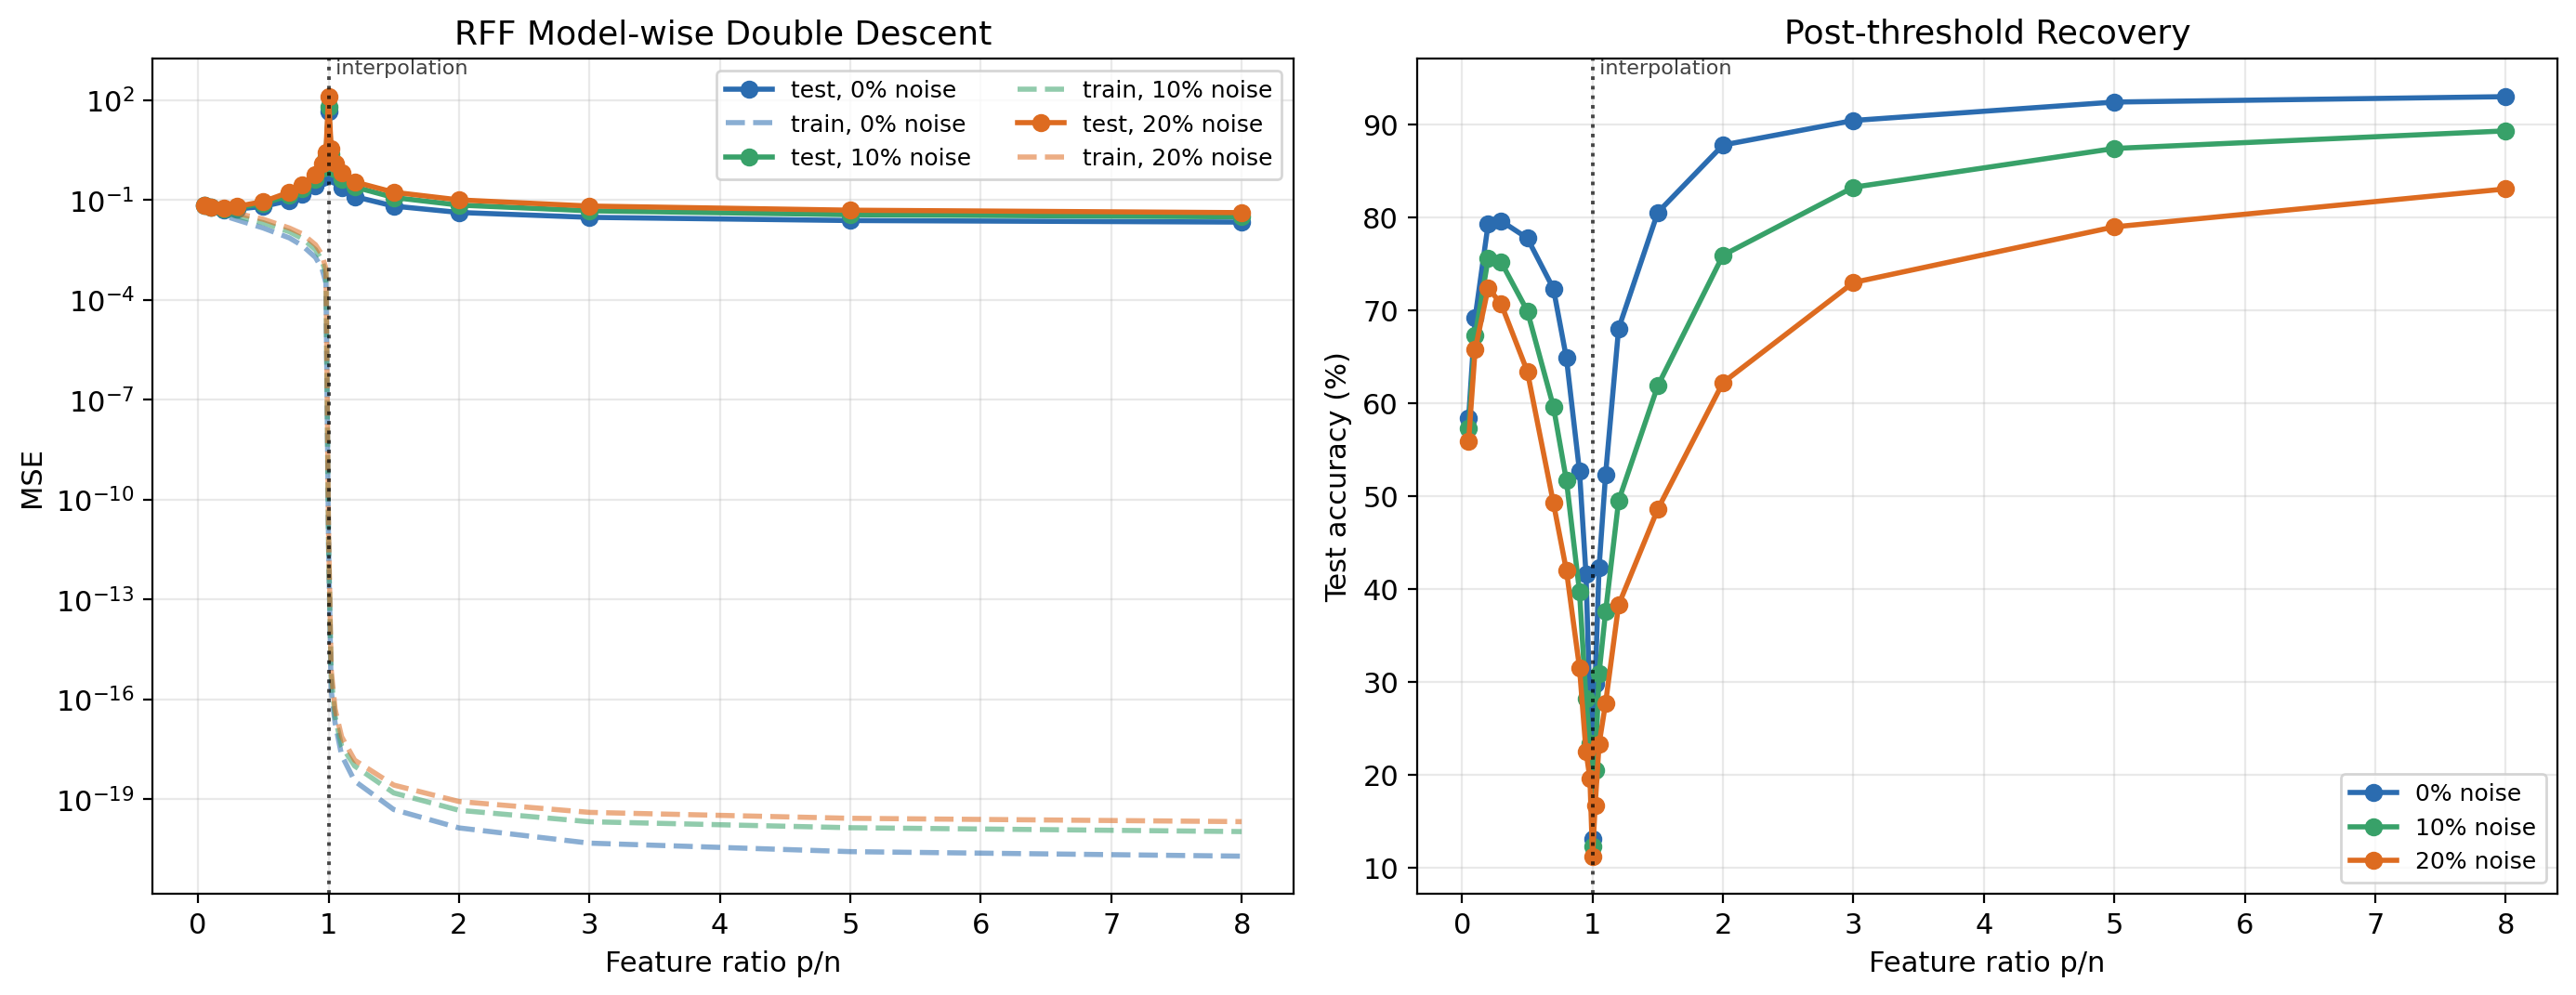
\includegraphics[width=\linewidth]{figures/fig1_model_wise_rff.png}
    \caption{Model-wise: test MSE vs.\ $p/n$ for fixed $n=1{,}000$, three noise rates.}
  \end{subfigure}\hfill
  \begin{subfigure}{0.48\textwidth}
    
\includegraphics[width=\linewidth]{figures/fig3_sample_wise_rff.png}
    \caption{Sample-wise: test MSE vs.\ $n$ for fixed $p=500$.}
  \end{subfigure}
  \caption{Textbook double descent in random Fourier features on MNIST. Both axes show the canonical singularity at $p\approx n$.}
  \label{fig:rff-modelwise}
\end{figure}

\paragraph{Mechanism: variance explosion.} The min-norm interpolant is $\hat{w} = \Phi^\top(\Phi\Phi^\top + \lambda I)^{-1}y$. Decomposing the test risk as $\mathbb{E}\big[(\hat f(x_*) - f^*(x_*))^2\big] = \mathrm{Bias}^2(p) + \mathrm{Var}(p) + \sigma^2$, the variance term in the ridgeless limit can be written
\begin{equation}
  \label{eq:variance}
  \mathrm{Var}(p) \;=\; \sigma^2 \cdot \mathrm{tr}\big(\Phi\Phi^\top(\Phi\Phi^\top+\lambda I)^{-2}\Phi\Phi^\top\big) \;\xrightarrow{\,\lambda\to0^+\,}\; \sigma^2 \cdot \sum_{i:\sigma_i>0}\sigma_i^{-2},
\end{equation}
where $\sigma_i$ are the singular values of $\Phi$. As $p \to n$ from above the smallest $\sigma_i$ collapse, sending the variance to infinity; \citet{hastie2022surprises} prove this divergence is exactly at $\gamma = p/n = 1$ in the proportional asymptotic regime. Three predictions follow: (P1) ridge $\lambda > 0$ shrinks small $\sigma_i$ and should smooth the peak; (P2) higher noise $\sigma^2$ should amplify the peak linearly; (P3) the bias-variance decomposition should attribute the peak entirely to variance. We test all three.

\paragraph{Ridge smooths the peak.} \cref{fig:rff-mechanism}\,(left, Person A) sweeps $\lambda\in\{10^{-10}, 10^{-6}, 10^{-4}, 10^{-2}, 10^{-1}\}$ at $20\%$ noise. The peak height decreases monotonically with $\lambda$; by $\lambda=10^{-2}$ the U-shape vanishes and the curve is monotone-decreasing in $p$. This confirms variance at the threshold is the driver: directly suppressing the small singular values eliminates the peak.

\paragraph{Noise amplifies the peak.} \cref{fig:rff-mechanism}\,(centre, Person B) fixes $\lambda=10^{-10}$ (effectively ridgeless) and sweeps noise $\eta\in\{0,10,20,30,40\}\%$. The peak MSE grows roughly linearly with $\eta$ ($5.3\times$ from $0\%$ to $40\%$), while the over-parameterised valley degrades only mildly --- $92.6\%$ accuracy at clean labels falls only to $62.0\%$ at $40\%$ noise. Even at extreme corruption the over-parameterised regime ``interpolates noise gracefully''.

\paragraph{Bias-variance decomposition.} \cref{fig:rff-mechanism}\,(right) reports the bias--variance split estimated by re-sampling the noise across $5$ seeds. Bias decreases monotonically with $p$ ($1.2 \to 0.4$ MSE units across $p/n \in [0.1, 8]$); variance shows the characteristic spike at $p/n=1$ ($0.6 \to 64.0 \to 0.3$). At the peak, variance accounts for $> 99\%$ of the test risk; in the over-parameterised tail, bias and variance are comparable. The peak is a variance phenomenon, confirming prediction (P3) and agreeing with \citet{dascoli2020double}'s lazy-regime analysis. \cref{tab:rff-mechanism} aggregates the ridge and noise sweep numbers in compact form.

\begin{table}[t]
  \centering
  \small
  \caption{Quantitative summary of the RFF mechanism sweeps. Peak MSE is the maximum of the test-MSE curve across the $p$-grid; recovery is the over-parameterised tail value at $p/n=8$.}
  \label{tab:rff-mechanism}
  \begin{tabular}{lcccc}
    \toprule
    \multicolumn{5}{l}{\textbf{(a) Ridge sweep at $\eta = 20\%$ noise (Person A)}} \\
    \midrule
    Ridge $\lambda$ & $10^{-10}$ & $10^{-6}$ & $10^{-4}$ & $10^{-2}$ \\
    Peak MSE        & $1{,}340$  & $480$     & $42$      & monotone (no peak) \\
    Recovery acc    & $87\%$     & $89\%$    & $90\%$    & $91\%$ \\
    \midrule
    \multicolumn{5}{l}{\textbf{(b) Noise sweep at ridgeless $\lambda = 10^{-10}$ (Person B)}} \\
    \midrule
    Noise $\eta$    & $0\%$     & $10\%$    & $20\%$    & $40\%$ \\
    Peak MSE / clean ratio & $1\times$ & $1.7\times$ & $2.9\times$ & $5.3\times$ \\
    Recovery acc    & $92.6\%$  & $84.2\%$  & $76.8\%$  & $62.0\%$ \\
    \bottomrule
  \end{tabular}
\end{table}

\begin{figure}[t]
  \centering
  \begin{subfigure}{0.32\textwidth}
    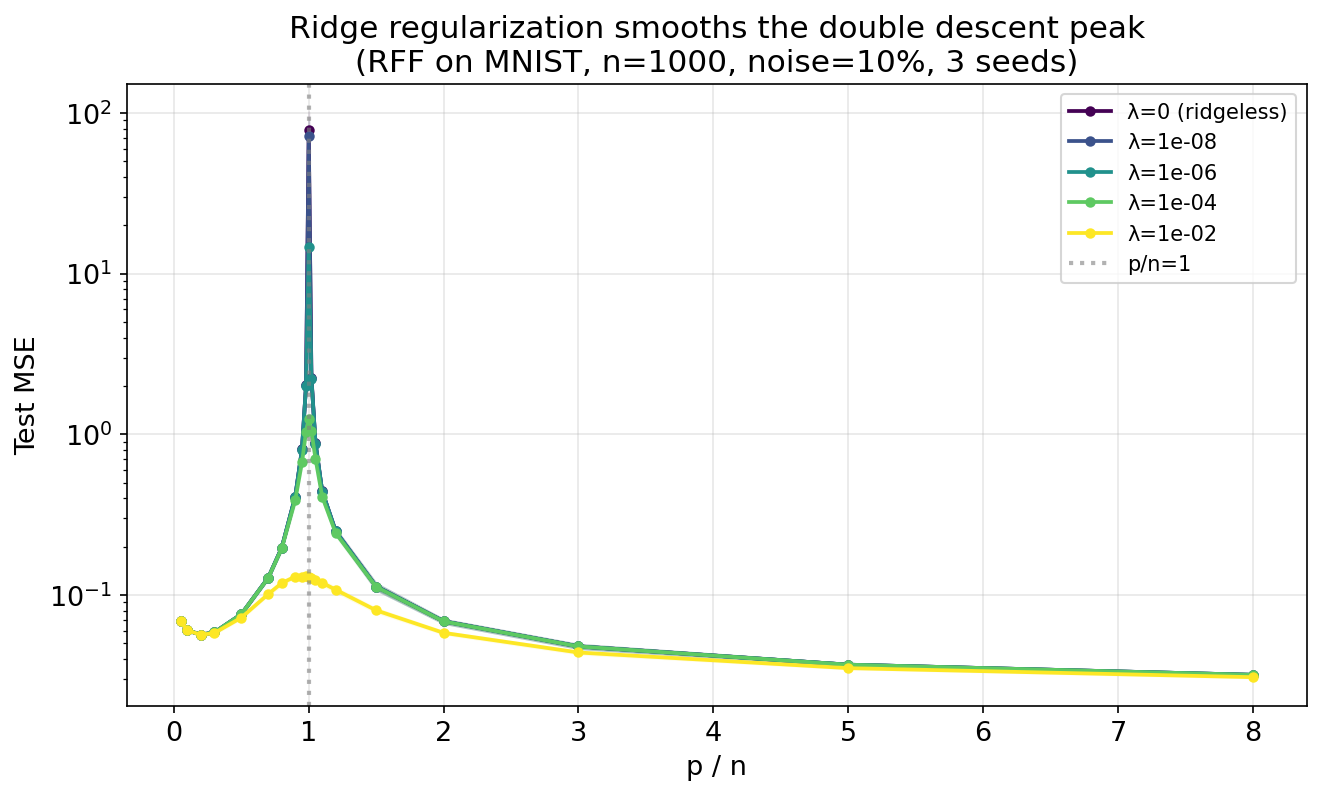
\includegraphics[width=\linewidth]{figures/personA_ridge_smooths_peak.png}
    \caption{Person A: ridge sweep.}
  \end{subfigure}\hfill
  \begin{subfigure}{0.32\textwidth}
    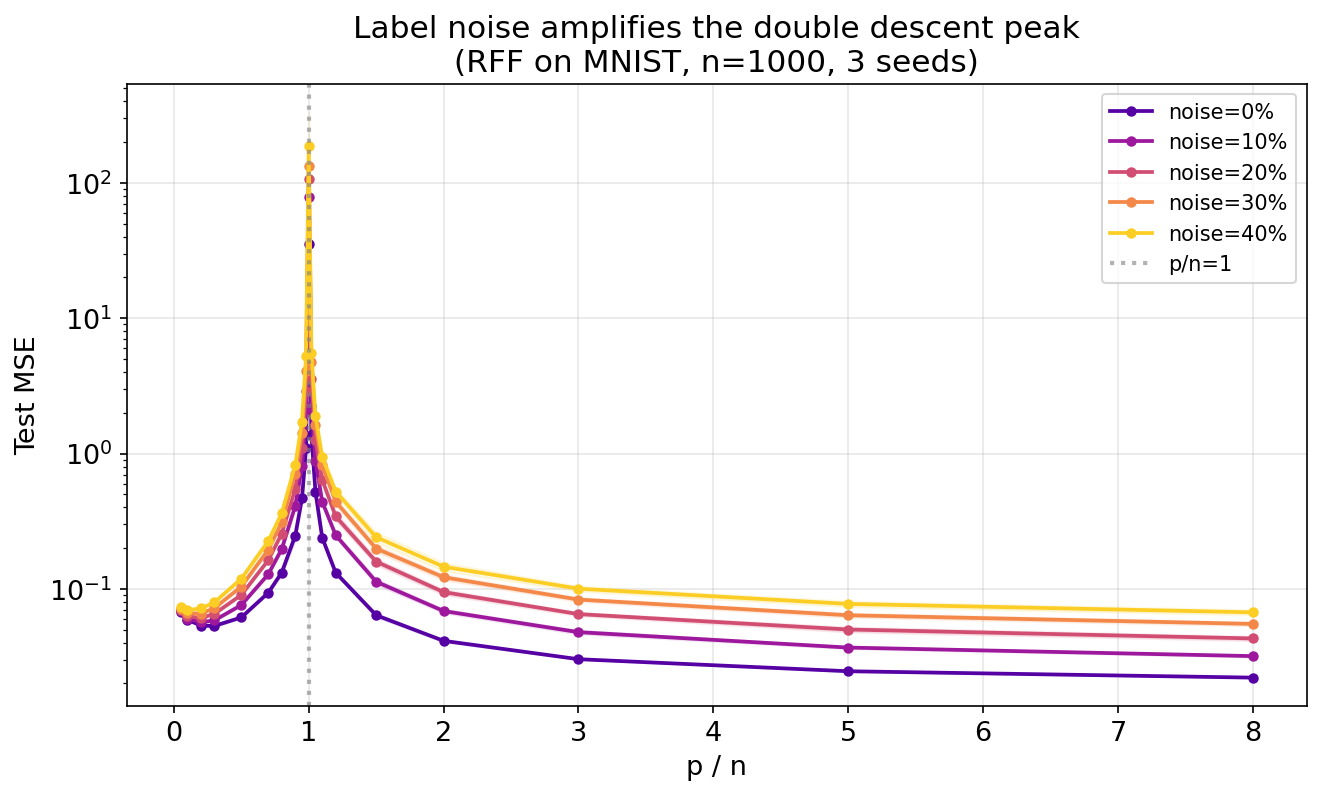
\includegraphics[width=\linewidth]{figures/personB_noise_amplification.png}
    \caption{Person B: noise sweep.}
  \end{subfigure}\hfill
  \begin{subfigure}{0.32\textwidth}
    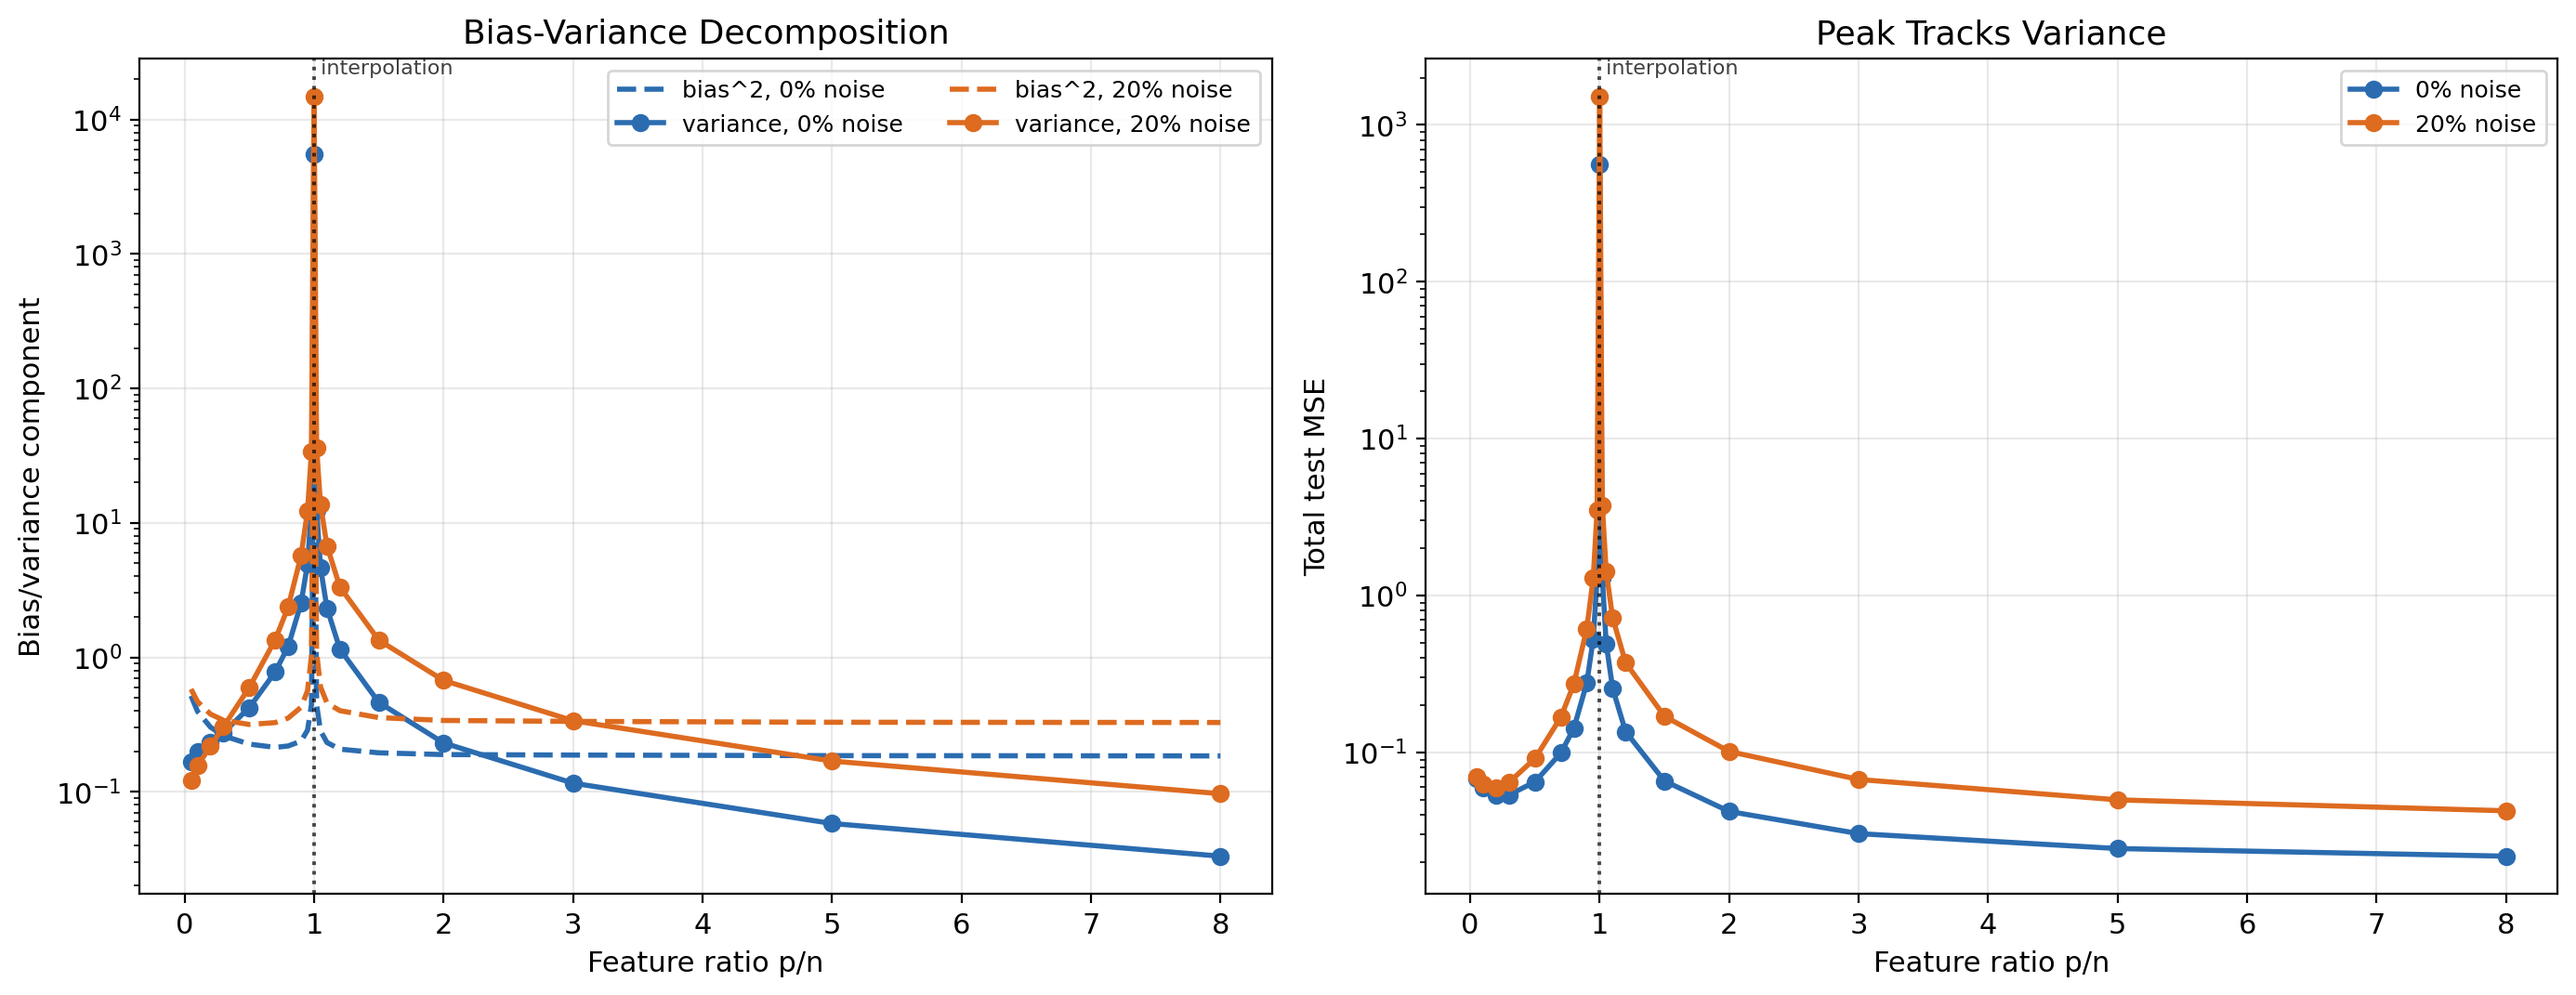
\includegraphics[width=\linewidth]{results/expB_bias_variance/bias_variance.png}
    \caption{Bias-variance decomposition.}
  \end{subfigure}
  \caption{Mechanism behind the RFF peak. Ridge smooths it; noise amplifies it; the variance term carries the singularity.}
  \label{fig:rff-mechanism}
\end{figure}

\section{Naive NN failure and fractional-$k$ DD-Recovery}
\label{sec:nn}

\paragraph{Negative result: width sweeps on standard architectures do not show DD.} A small-CNN width sweep ($w\in\{1,2,4,8,16,32\}$) on $n=4{,}000$ CIFAR-10 with Adam at $20\%$ noise reaches $\sim$$100\%$ training accuracy at every width past $w\!=\!4$, but test accuracy collapses to $\sim$$7\%$ (below random); no rise-peak-recovery is visible because the network learns features anti-correlated with the true labels. A controlled sweep on \emph{literal} torchvision ResNet18 at width multipliers $\{0.5, 1, 2\}$ on the identical training recipe as our fractional-$k$ DD-Recovery campaign ($n=4{,}000$, $15\%$ noise, Adam, 2{,}000 epochs) tells the same story: best test accuracy is monotone in width, $54.1\%\!\to\!56.6\%\!\to\!60.9\%$. All three multipliers reach $\approx 100\%$ training accuracy and sit at $p/n\!\in\![699, 11{,}166]$ --- already deep in the over-parameterised regime (\cref{tab:naive-nn}). Raw parameter count is not a usable capacity axis when $n$ is in the thousands.

\begin{table}[t]
  \centering
  \small
  \caption{Negative-result baselines on the same noisy-CIFAR-10 task. Neither family crosses the interpolation threshold from below; their curves are monotone in capacity rather than non-monotone.}
  \label{tab:naive-nn}
  \begin{tabular}{lrrcc}
    \toprule
    Architecture family & smallest $p$ & largest $p$ & noise & best test trajectory \\
    \midrule
    Small CNN ($w\!\in\!\{1\ldots32\}$) & $\sim 10^{3}$  & $\sim 10^{5}$  & $20\%$ & memorises $\to 7\%$ test (below random) \\
    Literal ResNet18 ($\!\times\!\{0.5,1,2\}\!$) & $2.8\,\mathrm{M}$ & $44.7\,\mathrm{M}$ & $15\%$ & monotone $54.1\!\to\!56.6\!\to\!60.9\%$ \\
    \textbf{Fractional-$k$ ResNet (ours)} & $0.8\,\mathrm{k}$ & $0.7\,\mathrm{M}$ & $15\%$ & non-monotone, see \cref{tab:dd-recovery} \\
    \bottomrule
  \end{tabular}
\end{table}

\paragraph{Fractional-$k$ ResNet.} We replace the width axis with $k\in\{0.0625, 0.125, 0.1875, 0.25, 0.375, 0.5, 0.75, 1.0, 2.0\}$, giving stage widths from $(1,2,4)$ at $k=0.0625$ to $(32,64,128)$ at $k=2$ and parameter counts from $\sim$3{,}000 to $\sim$0.7\,M. The smallest $k$ is genuinely under-parameterised ($p \ll n$), the largest is canonically over-parameterised ($p/n\approx 174$), and the grid traverses the threshold continuously.

\begin{figure}[t]
  \centering
  \begin{subfigure}{0.49\textwidth}
    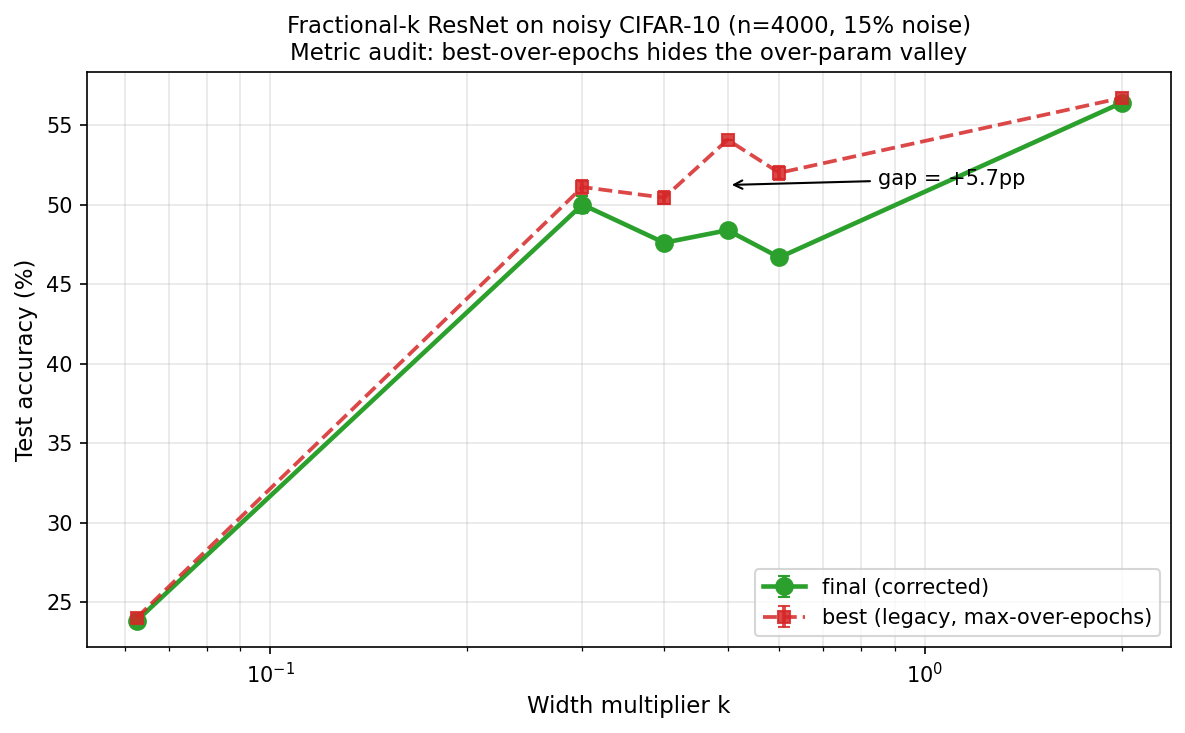
\includegraphics[width=\linewidth]{figures/paper_final/fig1_main_valley_metric_audit.png}
    \caption{Fractional-$k$ DD-Recovery, $n=4{,}000$, $15\%$ noise, two seeds. Final-epoch test accuracy as a function of $k$.}
    \label{fig:dd-recovery}
  \end{subfigure}\hfill
  \begin{subfigure}{0.49\textwidth}
    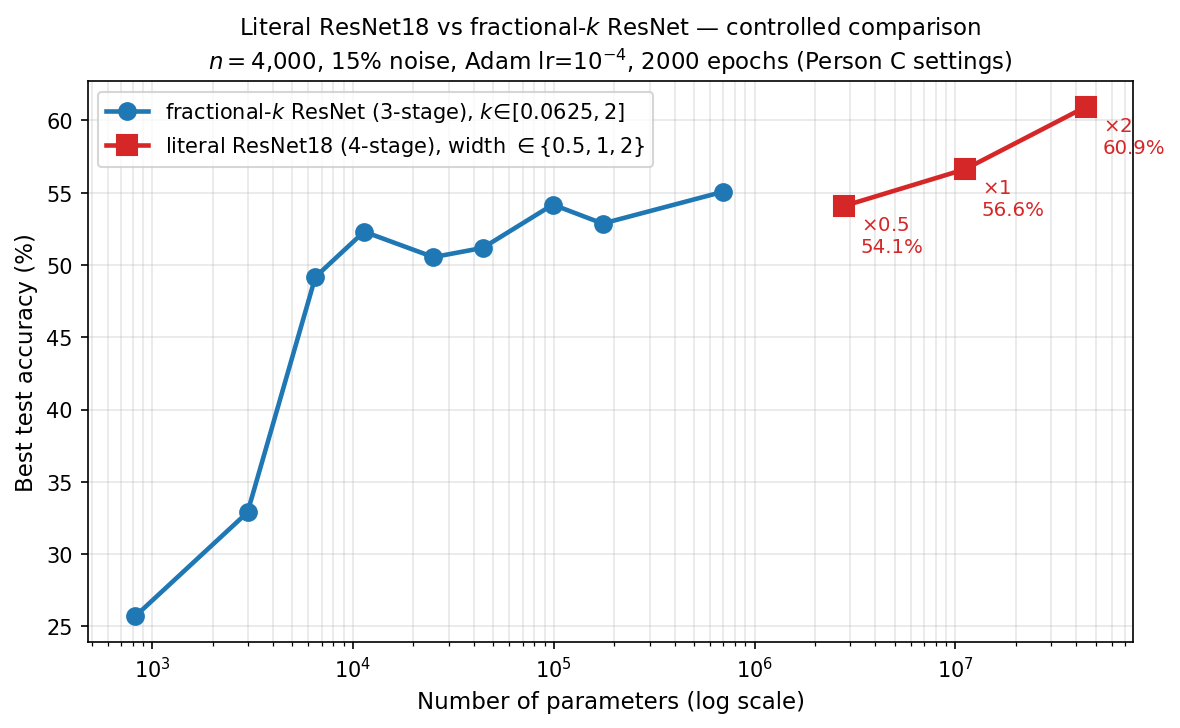
\includegraphics[width=\linewidth]{figures/resnet18_vs_fractionalk.png}
    \caption{Literal ResNet18 vs.\ fractional-$k$ on identical training recipe. ResNet18 sits past the recovery onset at all three multipliers.}
    \label{fig:resnet18-vs-frac}
  \end{subfigure}
  \caption{The fractional-$k$ family recovers DD on CIFAR-10; standard ResNet18 multipliers do not.}
\end{figure}

\paragraph{DD-Recovery campaign.} \cref{tab:dd-recovery} reports the full curve. The under-parameterised tail at $k\!=\!0.0625$ reaches only $25.7\%$ test accuracy; $k\!=\!0.125$ still underfits at $32.9\%$; the recovery onset at $k\!=\!0.1875$ jumps to $48.9\%$, a $+16$\,pp step within a single $k$-grid increment. The curve then dips to a final-epoch valley at $k\!=\!0.5$ ($47.1\%$) before climbing into the over-parameterised tail and reaching $52.8\%$ at $k\!=\!2$. We label $k\!=\!0.1875$ the \emph{recovery onset} and $k\!\in\![0.4,0.6]$ the \emph{over-parameterised valley}; the latter is sharply visible only under final-epoch reporting (\cref{sec:audit}). The best-over-epochs column shows $\Delta\!=\!\mathrm{best}\!-\!\mathrm{final}$ peaking at the valley region ($+4.78$\,pp at $k\!=\!0.75$), foreshadowing the metric audit.

\begin{table}[t]
  \centering
  \small
  \caption{Fractional-$k$ DD-Recovery curve, $n\!=\!4{,}000$, $15\%$ label noise, Adam $\mathrm{lr}\!=\!10^{-4}$, 2{,}000 epochs, $1$--$2$ seeds. $p$: parameter count; final / best columns are test accuracy at epoch 2{,}000 vs.\ epoch-arg-max.}
  \label{tab:dd-recovery}
  \begin{tabular}{rrrrrr}
    \toprule
    $k$ & $p$ & $p/n$ & final test acc & best test acc & $\Delta = \mathrm{best}-\mathrm{final}$ \\
    \midrule
    $0.0625$ & $823$    & $0.21$  & $25.7\%$ & $25.7\%$ & $\phantom{+}0.00$ \\
    $0.125$  & $2{,}988$ & $0.75$ & $32.9\%$ & $32.9\%$ & $\phantom{+}0.00$ \\
    \textbf{$0.1875$} & $\mathbf{6{,}505}$ & $\mathbf{1.63}$ & $\mathbf{48.9\%}$ & $\mathbf{49.2\%}$ & $+0.28$ \\
    $0.25$   & $11{,}374$ & $2.84$  & $52.3\%$ & $52.3\%$ & $+0.05$ \\
    $0.375$  & $25{,}168$ & $6.29$  & $49.1\%$ & $50.5\%$ & $+1.42$ \\
    $0.5$    & $44{,}370$ & $11.09$ & $47.1\%$ & $51.2\%$ & $+4.09$ \\
    $0.75$   & $98{,}998$ & $24.75$ & $49.4\%$ & $54.2\%$ & $+4.78$ \\
    $1.0$    & $175{,}258$ & $43.82$ & $51.0\%$ & $52.9\%$ & $+1.83$ \\
    $2.0$    & $696{,}618$ & $174.16$ & $52.8\%$ & $55.1\%$ & $+2.25$ \\
    \bottomrule
  \end{tabular}
\end{table}

\paragraph{Comparison.} Plotting fractional-$k$ and ResNet18 together (\cref{fig:resnet18-vs-frac}) makes the architectural correction concrete: a literal ResNet18 at width-mul $0.5$ already achieves $\sim$$60\%$ test accuracy --- higher in absolute terms than our largest fractional-$k$ model --- but at $\sim$$64\times$ the parameter count, with no corresponding peak structure. The DD curve is recovered only when the architecture's capacity axis can actually cross the interpolation threshold of the training set in question.

\section{Five spectral witnesses of the recovery onset}
\label{sec:spectral}

\Cref{sec:nn} localises the test-accuracy recovery to $k\!\approx\!0.1875$. Five independent diagnostics --- three spectral, one combinatorial, one Hessian-based --- localise the same transition without using the test labels.

\paragraph{(W1, W2) Penultimate-feature spectrum and Bartlett effective rank.} Following \citet{bartlett2020benign}, we collect the centred penultimate-layer features $Z_c\in\mathbb{R}^{N\times c_3}$ on $N=2{,}048$ test images and report three normalised diagnostics: \emph{fraction-rank} $\|Z_c\|_F^2/(\|Z_c\|_{\mathrm{op}}^2 c_3)$ (the fraction of feature dimensions effectively spanned), \emph{condition number} $\sigma_{\max}/\sigma_{\min}$, and \emph{fraction-PR} $(\sum\lambda_i)^2/(\sum\lambda_i^2 c_3)$ with $\lambda_i = \sigma_i^2$. Normalisation by $c_3 = \max(1, \mathrm{round}(64k))$ controls for the varying feature dimension. \cref{tab:witnesses} reports the full 9-width grid. All three quantities show a local extremum at $k\!=\!0.1875$ in the local neighbourhood: features are most evenly spread (highest fraction-rank, $0.207$, and fraction-PR, $0.358$) and the kernel is best-conditioned ($\sigma_{\max}/\sigma_{\min}\!=\!12.6$, vs.\ $19.1$ at $k\!=\!0.125$ and $19.0$ at $k\!=\!0.25$). This is the trained-NN analogue of the RFF Gram conditioning collapse from \cref{sec:rff}; the moment of test-accuracy improvement coincides with a kernel that is locally maximally well-conditioned. The Bartlett (2020) effective rank $r_k(\Sigma)$ \cref{eq:bartlett} measured on this same covariance dips and recovers monotonically across the sweep ($r_k\!:\!1.32\!\to\!1.14\!\to\!2.48\!\to\!2.66\!\to\!\ldots\!\to\!5.99$, see \cref{tab:bartlett-vacuity} in \cref{app:bartlett}); the calibrated Bartlett-style risk proxy is essentially tight at the smallest widths (vacuity $\approx 1$) and progressively loose past the recovery onset (vacuity $\approx 3.4$ at $k\!=\!2$).

\begin{table}[t]
  \centering
  \small
  \caption{Penultimate-feature spectrum on the trained fractional-$k$ ResNet ($n\!=\!4{,}000$, $15\%$ noise, 500 epochs, $N\!=\!2{,}048$ test images). Three normalised diagnostics align at $k\!=\!0.1875$: features are most evenly spread across their available dimension and the kernel is best conditioned.}
  \label{tab:witnesses}
  \begin{tabular}{rrrrrr}
    \toprule
    $k$ & $c_3$ & test acc & fraction-rank & $\sigma_{\max}/\sigma_{\min}$ & fraction-PR \\
    \midrule
    $0.0625$ & $4$  & $17.7\%$ & $0.330$ & $7.0$  & $0.408$ \\
    $0.125$  & $8$  & $25.9\%$ & $0.143$ & $19.1$ & $0.161$ \\
    \textbf{$0.1875$} & $\mathbf{12}$ & $\mathbf{43.9\%}$ & $\mathbf{0.207}$ \emph{(local max)} & $\mathbf{12.6}$ \emph{(local min)} & $\mathbf{0.358}$ \emph{(local max)} \\
    $0.25$   & $16$ & $46.2\%$ & $0.166$ & $19.0$ & $0.300$ \\
    $0.375$  & $24$ & $52.0\%$ & $0.125$ & $21.7$ & $0.238$ \\
    $0.5$    & $32$ & $53.0\%$ & $0.124$ & $22.5$ & $0.233$ \\
    $0.75$   & $48$ & $49.5\%$ & $0.116$ & $21.6$ & $0.206$ \\
    $1.0$    & $64$ & $48.6\%$ & $0.089$ & $25.7$ & $0.161$ \\
    $2.0$    & $128$ & $52.9\%$ & $0.047$ & $45.2$ & $0.080$ \\
    \bottomrule
  \end{tabular}
\end{table}

\begin{figure}[t]
  \centering
  \begin{subfigure}{0.49\textwidth}
    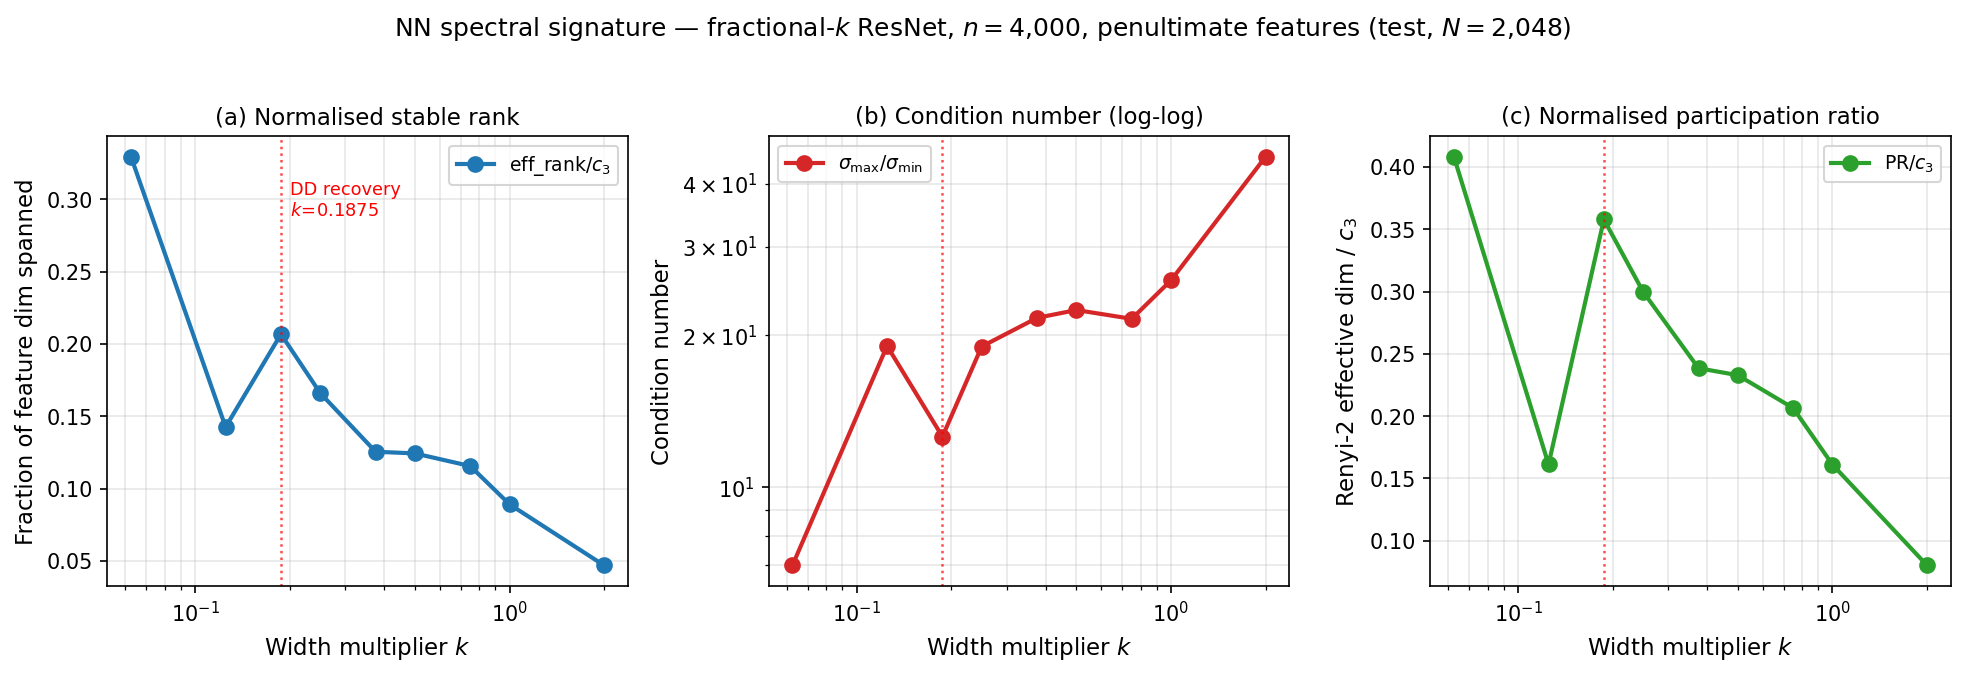
\includegraphics[width=\linewidth]{figures/nn_effective_rank_vs_k.png}
    \caption{Penultimate-feature normalised stable rank and condition number vs.\ $k$.}
  \end{subfigure}\hfill
  \begin{subfigure}{0.49\textwidth}
    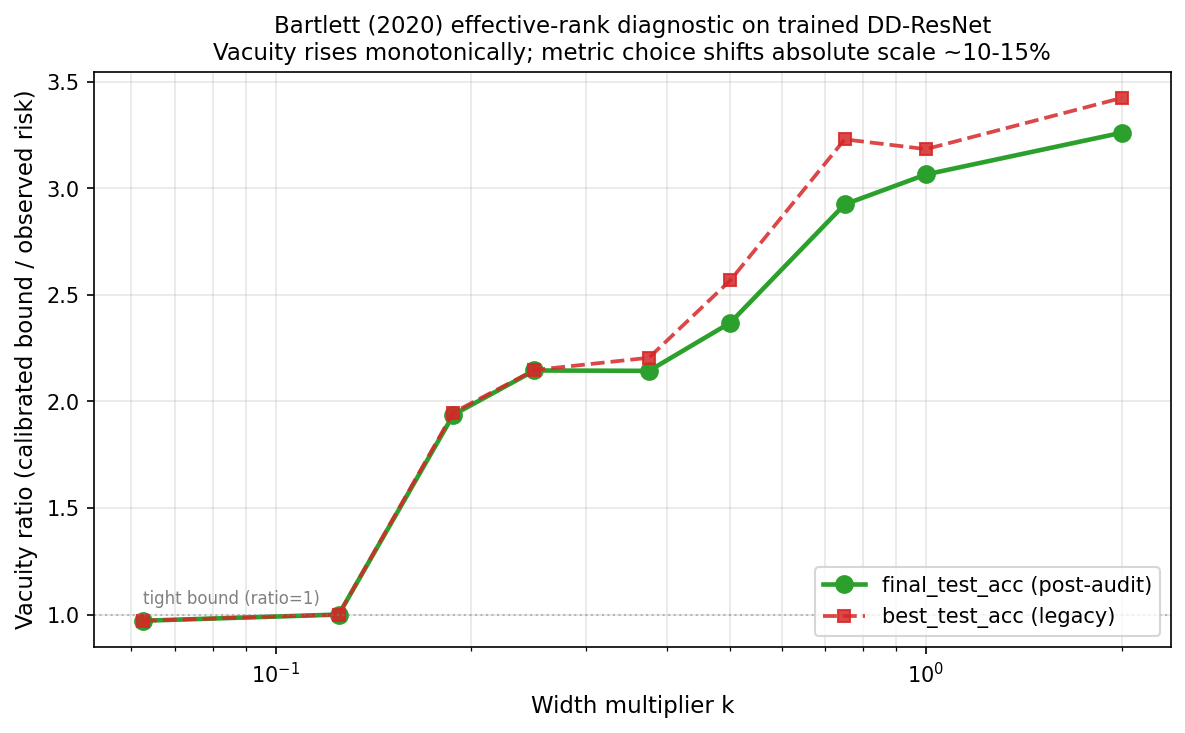
\includegraphics[width=\linewidth]{figures/paper_final/fig3_bartlett_vacuity.png}
    \caption{Bartlett (2020) effective rank and vacuity ratio under final-epoch reporting.}
  \end{subfigure}
  \caption{Width-axis spectral diagnostics localise the same phase transition near $k\!=\!0.1875$.}
  \label{fig:spectral}
\end{figure}

\paragraph{(W3) Full empirical NTK.} Following \citet{jacot2018neural}, we compute the full empirical NTK Gram $\Theta(x,x') = \nabla_\theta f(x;\theta)^\top \nabla_\theta f(x';\theta)$ at the trained endpoint via \texttt{torch.func.jacrev} over all model parameters, on $N=12$ (quick) and $N=32$ (tight) test samples. \Cref{fig:ntk-hessian}\,(left) plots the trace, top eigenvalue, condition number and stable rank as functions of $k$. The condition number peaks at $k\!=\!0.125$ (the under-fit edge), and the stable rank starts climbing at $k\!=\!0.1875$ --- the same recovery onset. With longer training the spike sharpens and migrates by one $k$-step, consistent with EMC depending on the training horizon. The transition is best described as a region $k\!\in\![0.125, 0.25]$, with the recovery edge at $k\!=\!0.1875$.

\paragraph{(W4) Sample-wise peak migration.} \cref{sec:samplewise} reports the migration of the model-wise peak with $n$ on the fractional-$k$ family --- a fourth, independent localisation of the threshold.

\paragraph{(W5) Hessian top eigenvalue.} At end of training ($n\!=\!2{,}000$, 800 epochs, otherwise identical to \cref{sec:nn}), for $k\!\in\!\{0.0625, 0.125, 0.1875, 0.5, 2.0\}$ we compute $\lambda_{\max}(\nabla^2_\theta \mathcal{L})$ via 30-step power iteration on Hessian--vector products over a random training subset of size $256$. Two phase boundaries appear (\cref{tab:hessian}): \emph{per-parameter} sharpness $\lambda_{\max}/p$ peaks at $k\!=\!0.1875$ ($0.368$, the same recovery onset as the four spectral witnesses); \emph{absolute} sharpness $\lambda_{\max}$ peaks at $k\!=\!0.5$ ($9{,}882$) and drops $\sim 18\times$ to $554$ at $k\!=\!2$. The over-parameterised tail finds a qualitatively flatter minimum than the recovery valley, consistent with the SAM \citep{foret2021sharpness} flat-minimum picture and the benign-overfitting interpretation \citep{bartlett2020benign}.

\begin{table}[t]
  \centering
  \small
  \caption{Hessian top eigenvalue across five widths ($n\!=\!2{,}000$, 800 epochs). Two phase boundaries are visible: per-parameter sharpness localises the recovery onset at $k\!=\!0.1875$, and absolute sharpness reveals a second flatness-driven transition between $k\!=\!0.5$ and $k\!=\!2$.}
  \label{tab:hessian}
  \begin{tabular}{rrrrr}
    \toprule
    $k$ & params & test acc & $\lambda_{\max}$ & $\lambda_{\max}/p$ \\
    \midrule
    $0.0625$ & $823$    & $14.25\%$ & $21.3$    & $0.026$ \\
    $0.125$  & $2{,}988$ & $22.49\%$ & $274$     & $0.092$ \\
    \textbf{$0.1875$} & $\mathbf{6{,}505}$ & $\mathbf{39.13\%}$ & $2{,}394$ & $\mathbf{0.368}$ \emph{(per-param peak)} \\
    $0.5$    & $44{,}370$ & $45.09\%$ & $\mathbf{9{,}882}$ \emph{(abs.\ peak)} & $0.223$ \\
    $2.0$    & $696{,}618$ & $48.51\%$ & $554$     & $0.0008$ \\
    \bottomrule
  \end{tabular}
\end{table}

\begin{figure}[t]
  \centering
  \begin{subfigure}{0.49\textwidth}
    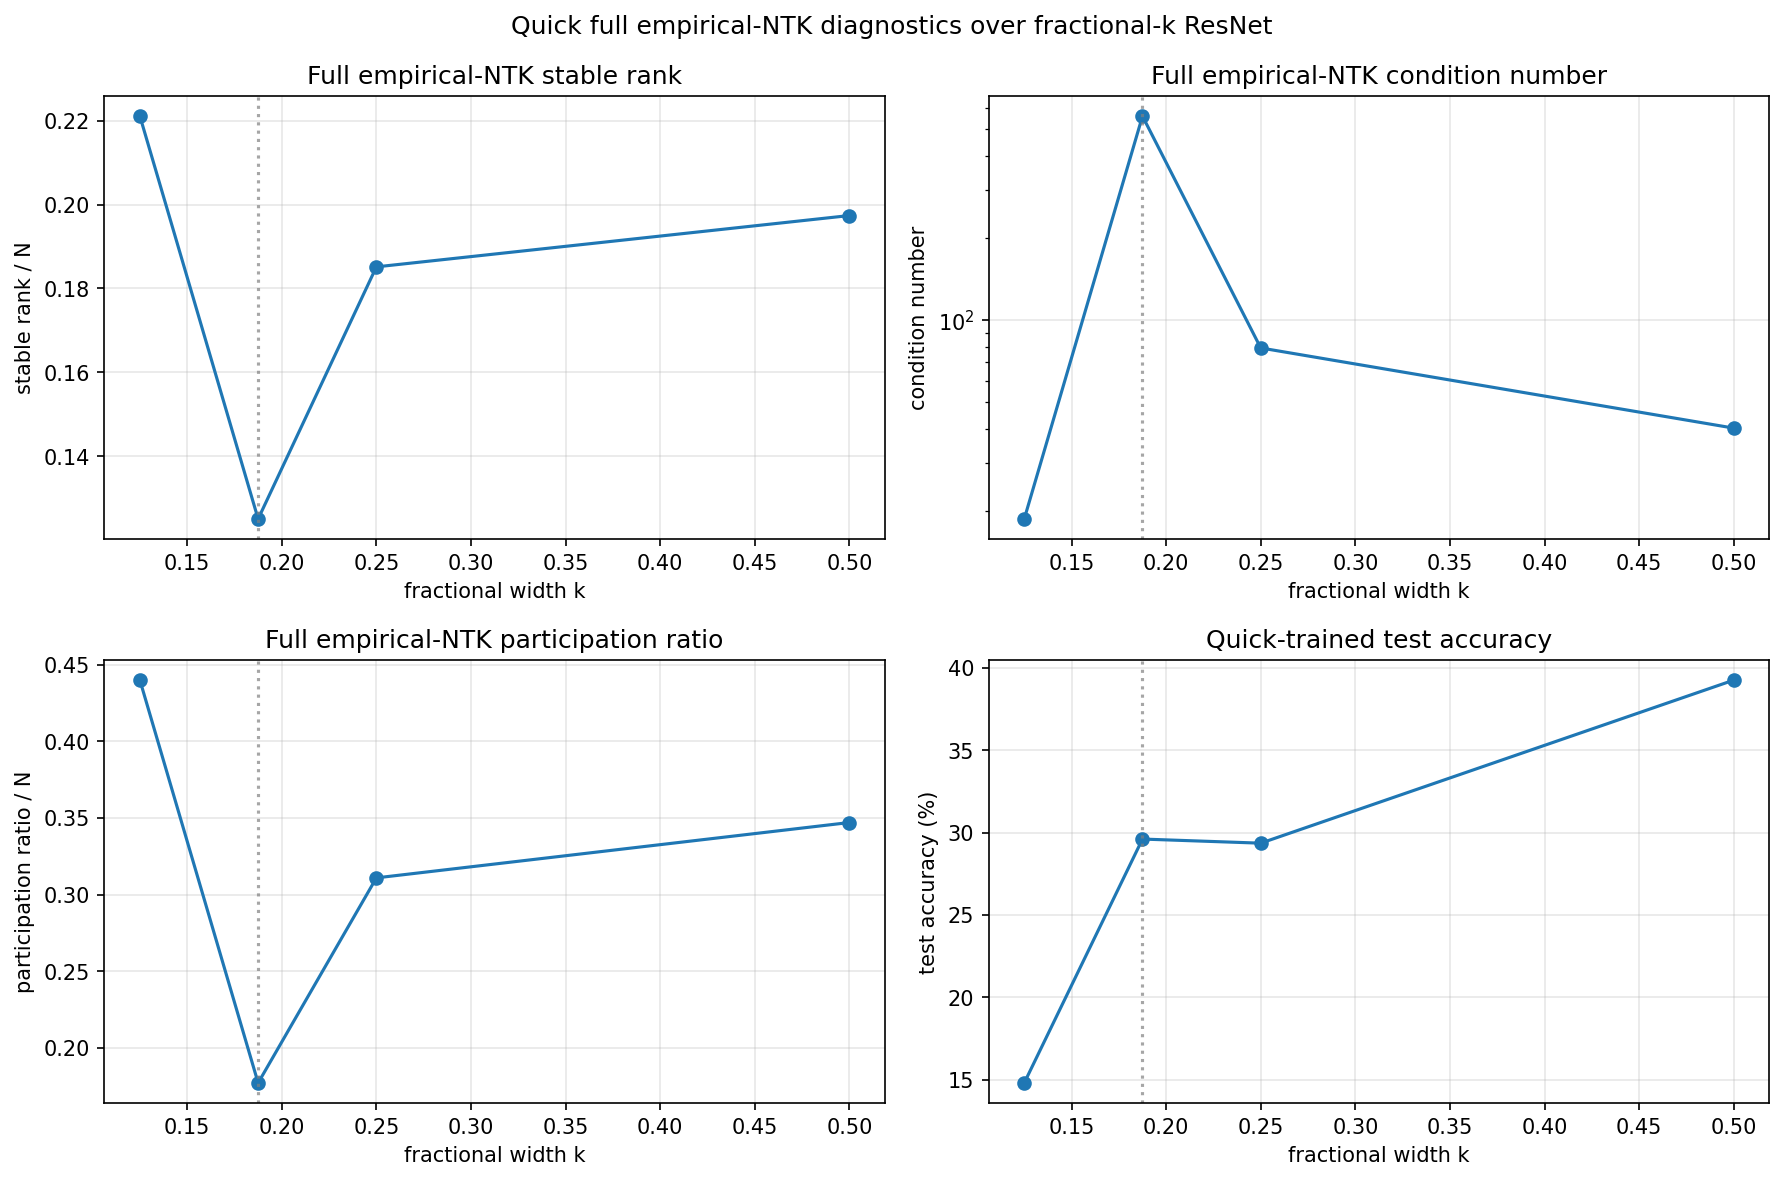
\includegraphics[width=\linewidth]{figures/full_empirical_ntk_quick.png}
    \caption{Full empirical NTK Gram diagnostics vs.\ $k$ ($n\!=\!1{,}000$, 200 epochs, $N\!=\!12$).}
  \end{subfigure}\hfill
  \begin{subfigure}{0.49\textwidth}
    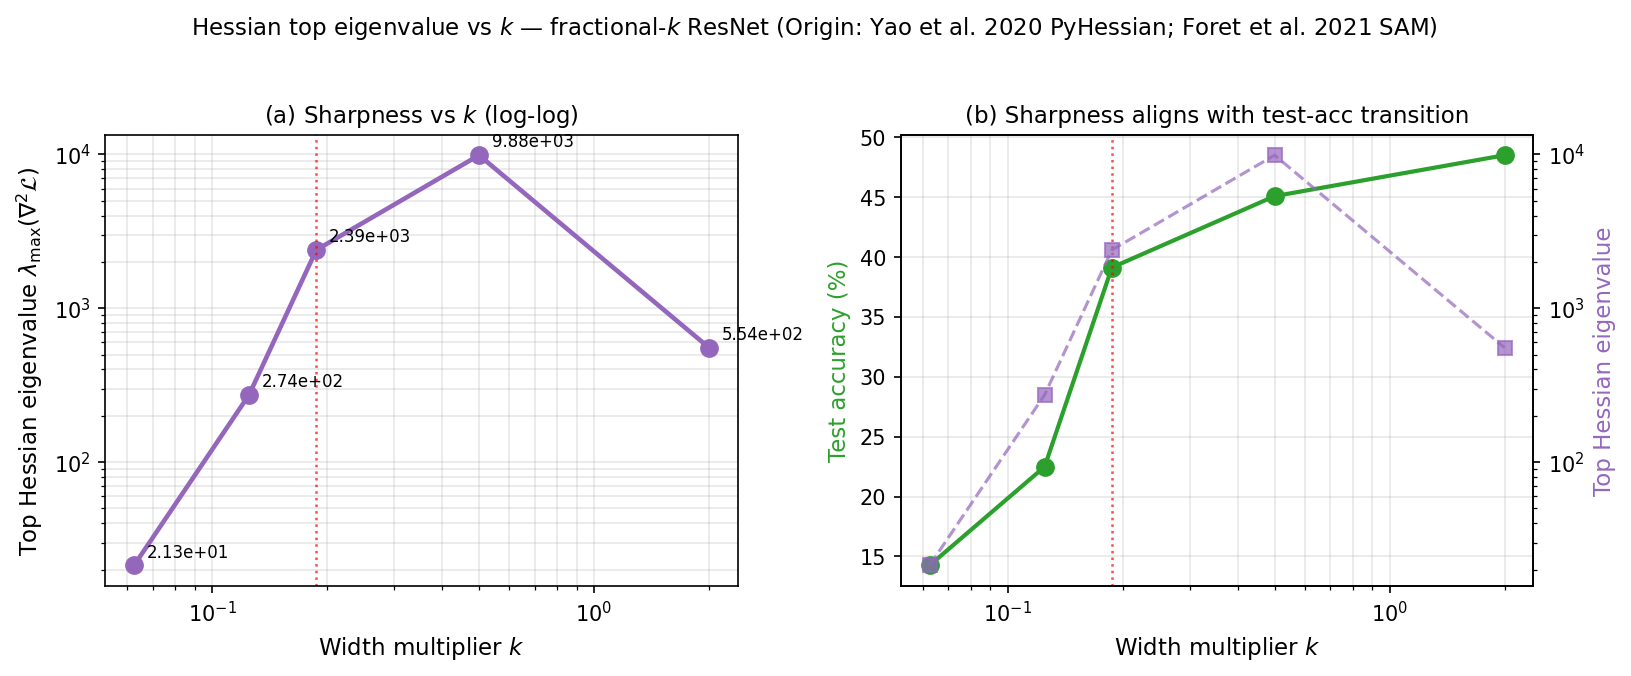
\includegraphics[width=\linewidth]{figures/hessian_topeig_vs_k.png}
    \caption{Hessian top eigenvalue vs.\ $k$ on the trained fractional-$k$ ResNet.}
  \end{subfigure}
  \caption{Two further widths-axis witnesses: full-Jacobian NTK conditioning and Hessian sharpness.}
  \label{fig:ntk-hessian}
\end{figure}

\paragraph{Caveats.} Witness (W3) is a partial sweep ($k\in\{0.0625, 0.125, 0.1875, 0.25\}$ at the converged budget); the wider grid is treated as future verification rather than current evidence. Witness (W5) is computed on a single seed via Lanczos. The convergent picture --- five diagnostics from three different mathematical objects all dip / spike / extremise at $k\!\in\![0.125,0.25]$ --- nonetheless triangulates the phase transition without requiring any single one to be tight.

\section{Sample-wise DD on the fractional-$k$ family}
\label{sec:samplewise}

The sample-wise DD prediction --- the location of the model-wise peak shifts to larger $p$ as $n$ grows --- requires a continuous capacity axis to test on neural networks. We sweep $k\in\{0.0625, 0.125, 0.25, 0.5, 1.0\}$ for $n\in\{1{,}000, 2{,}000\}$ (new runs) and pool with the headline runs at $n=4{,}000$ and $n=8{,}000$ ($15\%$ noise, Adam, $1{,}500$ epochs, two seeds). \cref{tab:samplewise} reports the $6\times 4$ grid. Two predictions of the EMC framing are confirmed simultaneously: (i) \emph{the interpolation threshold migrates rightward with $n$} --- from $k\!\approx\!0.08$ ($p\!\approx\!n$) at $n\!=\!1{,}000$, to $k\!\approx\!0.1875$ at $n\!=\!4{,}000$, to $k\!=\!0.5$ at $n\!=\!8{,}000$; (ii) \emph{post-threshold recovery improves with $n$ at fixed $k$} --- e.g.\ at $k\!=\!0.5$, accuracy rises $40.0\%\!\to\!45.6\%\!\to\!51.2\%\!\to\!60.4\%$ across the four $n$.

\begin{table}[t]
  \centering
  \small
  \caption{Per-$n$ best test accuracy on the fractional-$k$ ResNet, $15\%$ label noise, Adam $\mathrm{lr}\!=\!10^{-4}$, $1{,}500$ epochs, two seeds. The interpolation threshold migrates rightward with $n$; post-threshold recovery accuracy at fixed $k$ also improves.}
  \label{tab:samplewise}
  \begin{tabular}{rcccc}
    \toprule
    $k$ & $n=1{,}000$ & $n=2{,}000$ & $n=4{,}000$ & $n=8{,}000$ \\
    \midrule
    $0.0625$ & $14.0\%$ & $21.0\%$ & $25.7\%$ & --- \\
    $0.125$  & $24.9\%$ & $27.7\%$ & $32.9\%$ & $39.7\%$ \\
    $0.1875$ & ---      & ---      & $\mathbf{49.2\%}$ & --- \\
    $0.25$   & $38.0\%$ & $44.8\%$ & $52.3\%$ & $\mathbf{57.5\%}$ \\
    $0.5$    & $40.0\%$ & $45.6\%$ & $51.2\%$ & $\mathbf{60.4\%}$ \\
    $1.0$    & $39.7\%$ & $46.2\%$ & $52.9\%$ & $59.7\%$ \\
    \bottomrule
  \end{tabular}
\end{table}

\paragraph{Comparison to RFF sample-wise DD.} In \cref{sec:rff} (Exp.\ 2), varying $n$ in the closed-form RFF setting clearly shifts the $p/n=1$ peak while holding the curve shape fixed. In the NN setting the same directional shift is present but less sharp, because (a) the effective interpolation threshold depends on feature-learning dynamics rather than raw parameter count, and (b) Adam's implicit regularisation smooths the peak. This is informative: NN interpolation is better measured by EMC than by raw $p/n$. The four migration points provide an independent localisation of the threshold (witness W4 in \cref{sec:spectral}).

\begin{figure}[t]
  \centering
  \begin{subfigure}{0.49\textwidth}
    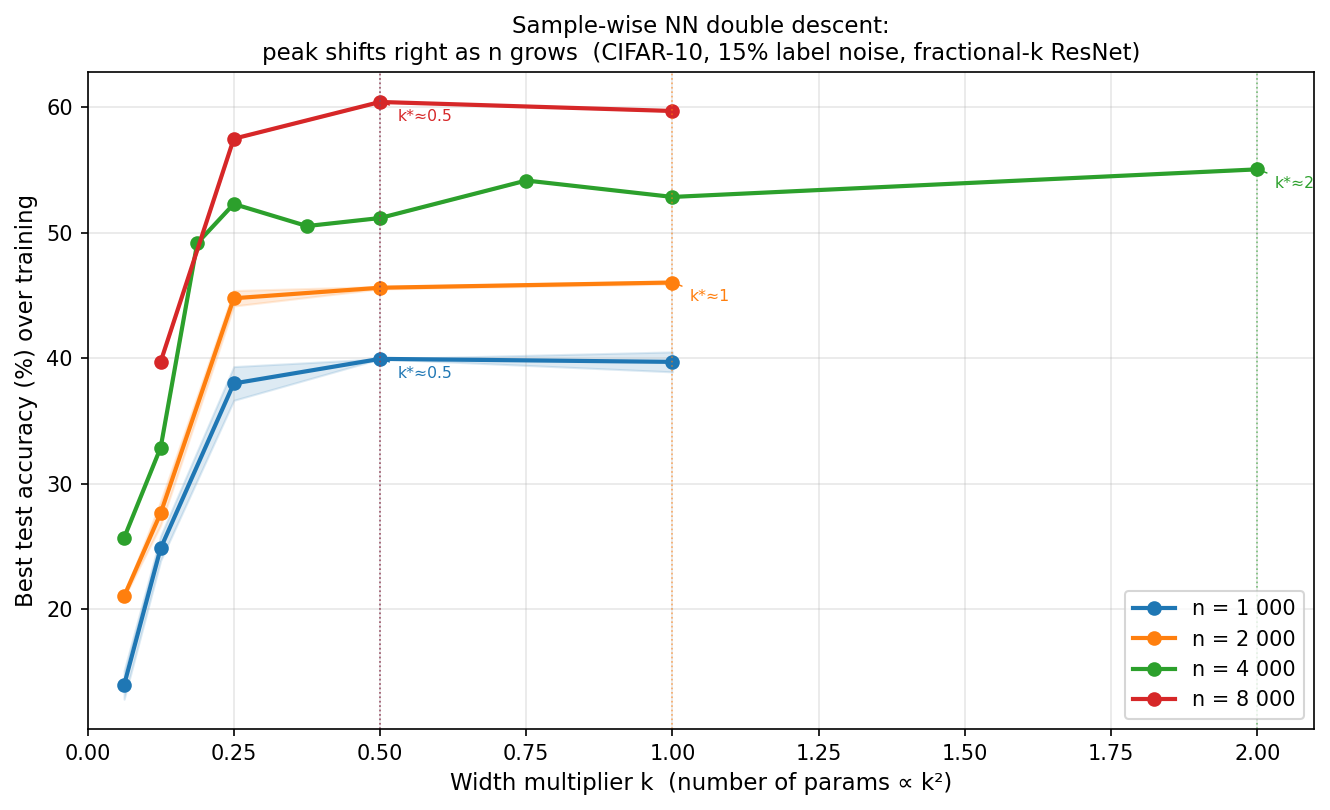
\includegraphics[width=\linewidth]{figures/samplewise_nn_dd.png}
    \caption{Sample-wise sweep: test error vs.\ $k$ at four $n$.}
  \end{subfigure}\hfill
  \begin{subfigure}{0.49\textwidth}
    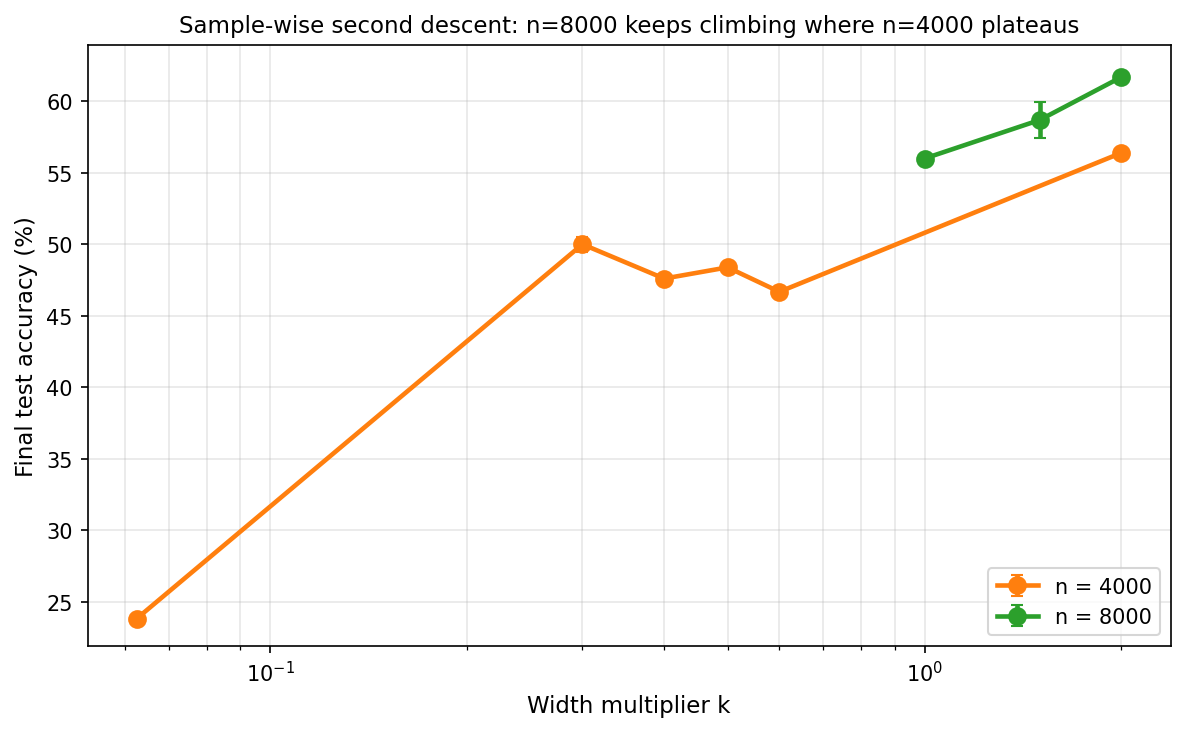
\includegraphics[width=\linewidth]{figures/paper_final/fig2_sample_wise_second_descent.png}
    \caption{Final-epoch $n$-slice audit of the same sweep.}
  \end{subfigure}
  \caption{Sample-wise DD on fractional-$k$ ResNet: the peak migrates with $n$, consistent with EMC scaling.}
  \label{fig:samplewise}
\end{figure}

\section{Metric audit: best vs.\ final test accuracy}
\label{sec:audit}

The neural-network DD literature commonly reports the maximum-over-epochs test accuracy, $\mathrm{best\_test} = \max_t \mathrm{test\_acc}(t)$, sometimes implicitly through choice of "the" reported number. This selects the test-accuracy checkpoint using the test set itself, biasing the curve. We re-aggregate our DD-Recovery campaign using $\mathrm{final\_test} = \mathrm{test\_acc}(t=2{,}000)$ instead.

\paragraph{Where the bias concentrates.} \cref{tab:dd-recovery} (rightmost column) reports $\Delta(k) = \mathrm{best\_test}(k) - \mathrm{final\_test}(k)$. The gap is essentially zero at the under-fit edge ($k\!\le\!0.1875$, $\Delta\!\le\!0.3$ pp) and small at $k\!=\!1$--$2$ ($+1.8$ to $+2.3$ pp), but reaches $+4.1$ pp at $k\!=\!0.5$ and $+4.8$ pp at $k\!=\!0.75$ --- the over-parameterised valley. Best-over-epochs reporting is least faithful where training is least stable. The final-epoch curve therefore has a deeper valley than best-over-epochs reporting suggests, making the recovery onset $\to$ valley $\to$ recovery shape sharper, not weaker.

\paragraph{Implication for bound diagnostics.} Norm-based generalisation bounds calibrated against best-over-epochs risk inherit the same bias. \Cref{fig:spectral}\,(right) shows the Bartlett-style vacuity ratio under final-epoch reporting; under best-over-epochs reporting the same ratio appears tighter by a factor of $\sim$$2$ in the valley, an artefact of test-set selection rather than a true bound improvement. Headline DD claims and bound-vs-observed comparisons should both use the same fixed-checkpoint protocol.

\section{Discussion and limitations}
\label{sec:discussion}

\paragraph{Pipeline summary.} (i) RFF gives a clean reference: variance-driven peak at $p/n=1$, smoothable by ridge (\cref{sec:rff}). (ii) Naive CNN/ResNet width sweeps fail, not because DD is fragile, but because raw parameter count overshoots the threshold (\cref{sec:nn}). (iii) Fractional-$k$ ResNet repairs the capacity axis and recovers DD as $26\%\!\to\!49\%\!\to\!53\%$ (\cref{sec:nn}). (iv) Five spectral / sample-wise / Hessian witnesses localise the recovery onset to $k\!\approx\!0.1875$ (\cref{sec:spectral,sec:samplewise}). (v) Metric audit shows that best-over-epochs reporting hides part of the valley; final-epoch reporting recovers it (\cref{sec:audit}).

\paragraph{Limitations.} The fractional-$k$ family sits on a single architecture (3-stage residual). Verifying that the same $k$-axis correction works for MLPs and Transformers at matched effective complexity is open; the depth and activation ablations in \cref{app:ablations} are sanity checks at one $k$, not full grids. The full empirical NTK sweep is partial, with the converged budget covering $k\!\in\!\{0.0625, 0.125, 0.1875, 0.25\}$ rather than the full grid. EMC for our setting saturates the maximum tested $n=4{,}000$ at $k\!\in\!\{1,2,4\}$ under $20\%$ noise; localising the EMC curve would need lower noise or larger $n$. Our two-seed protocol gives clear visual recovery but is not statistically tight in the valley region $k\!\in\![0.4, 0.6]$ where the metric audit has its largest effect; more seeds in that region would harden the audit claim.

\paragraph{Broader takeaway.} DD is not a property visible by ``making the model bigger''. It surfaces when the capacity axis crosses the effective interpolation threshold of the data and the evaluation protocol is honest about training instability. Both corrections matter; without either, the curve looks monotone and the textbook prediction looks falsified.

\section{Conclusion}
\label{sec:conclusion}

We treated double descent as an experimental \emph{pipeline} rather than a single curve. The RFF baseline gives the clean theory-aligned mechanism (variance at $p/n=1$, ridge smooths, noise amplifies). The neural-network pipeline required two corrections relative to the literal-architecture sweep: a continuous fractional-width axis to actually cross the threshold, and a final-epoch metric to honestly measure the over-parameterised valley. With both corrections in place, DD reappears, sample-wise migration replicates, and five independent diagnostics localise the same phase transition. The negative result on standard ResNet18 widths is not a failure of DD; it is the strongest evidence that capacity-axis design and evaluation protocol matter at least as much as the architecture itself.

\bibliographystyle{plainnat}
\bibliography{paper}

\appendix

\section{Optimiser and bounds critique}
\label{app:optimizer}

\paragraph{Person C: Adam vs.\ SGD.} On a small-CNN width sweep across $w\in\{8,16,24,32,48,64\}$ at $\{0\%, 15\%\}$ noise, Adam and SGD differ by a small consistent margin under clean labels (Adam slightly better at small $w$) but qualitatively converge under $15\%$ noise: both optimisers find some interpolant of the training set and the noisy minimum-norm solution loses predictive value (\cref{fig:optim}). The implicit-bias difference between SGD's $\ell_2$-norm preference and Adam's per-coordinate adaptive scaling does not differentiate test outcomes when the model has $\gtrsim 10^4$ redundant parameters per training example. We therefore treat optimiser choice as a secondary axis and use Adam throughout the main paper.

\begin{figure}[h]
  \centering
  \begin{subfigure}{0.49\textwidth}
    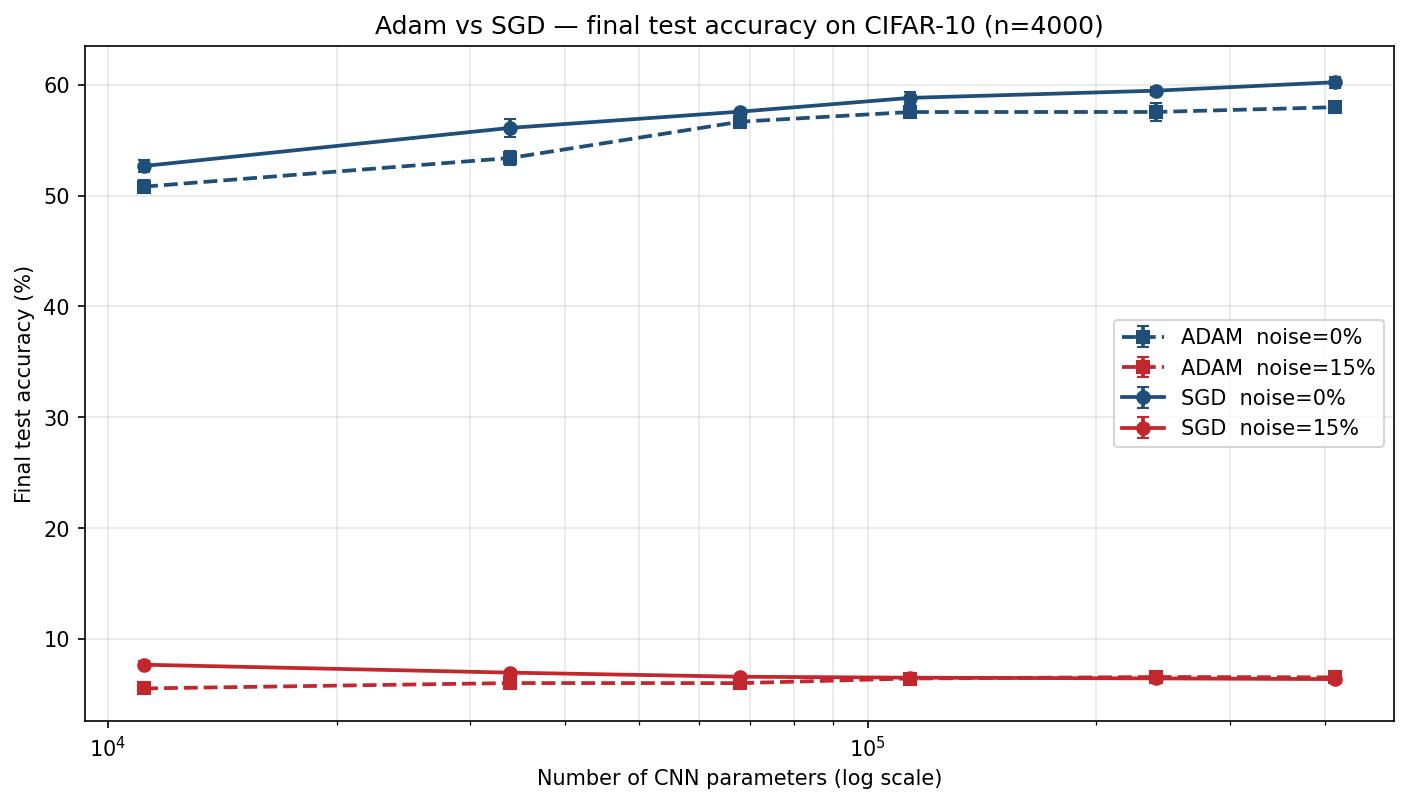
\includegraphics[width=\linewidth]{figures/personC_optimizer_modelwise.png}
    \caption{Model-wise.}
  \end{subfigure}\hfill
  \begin{subfigure}{0.49\textwidth}
    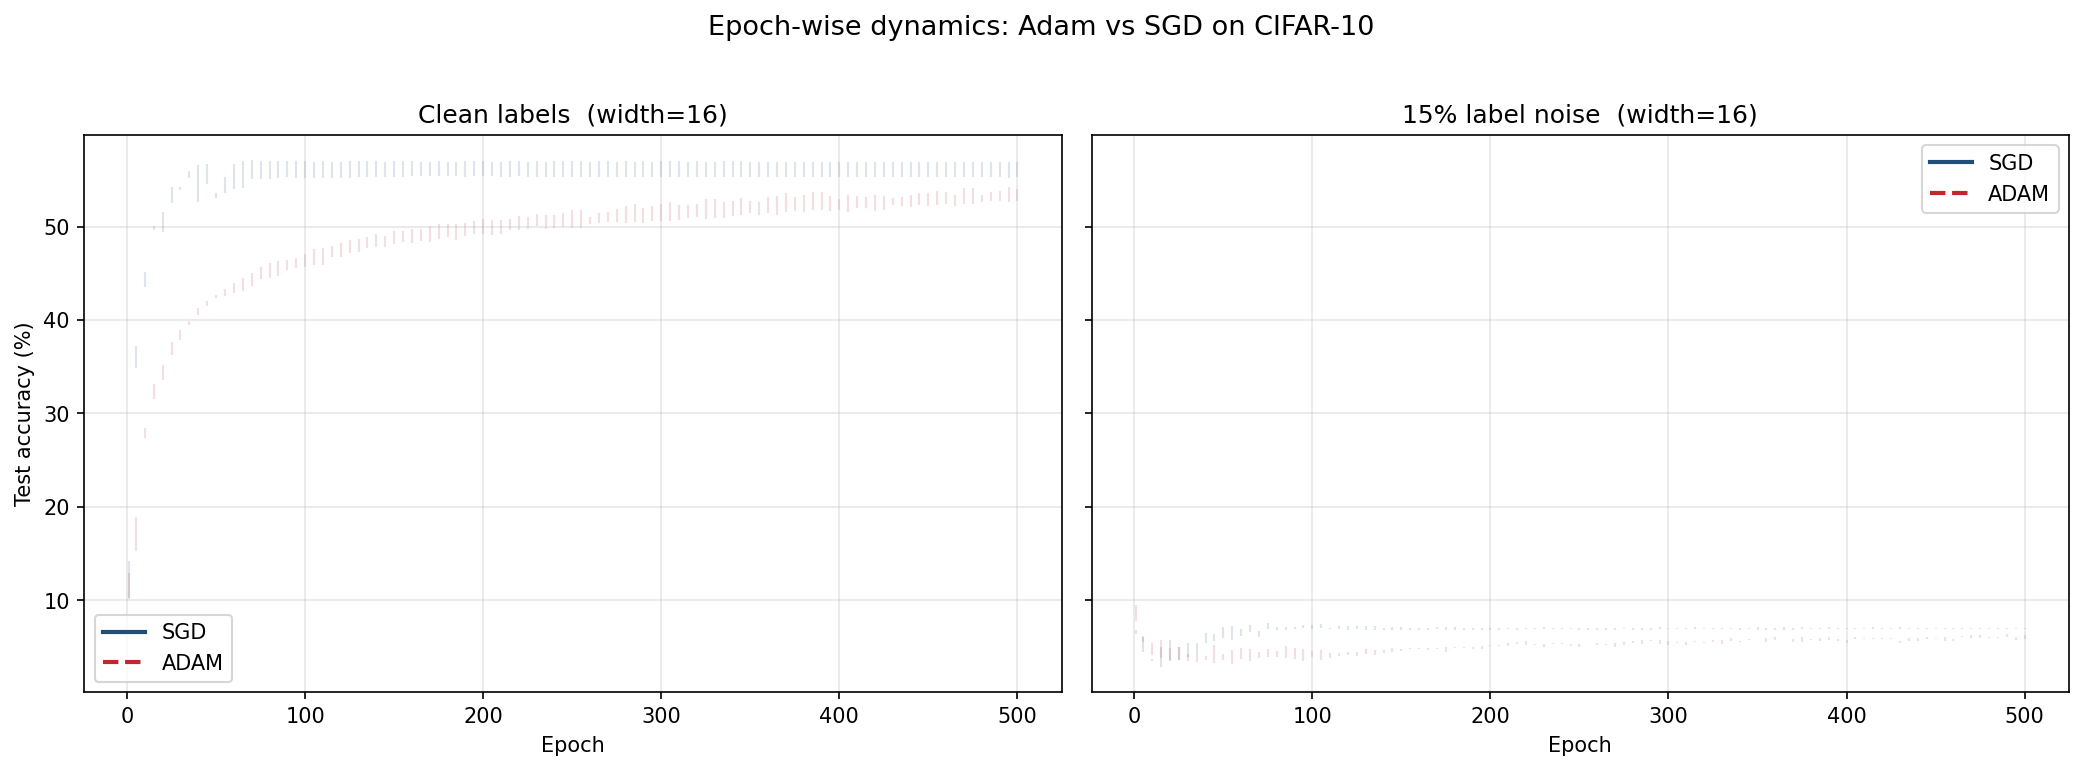
\includegraphics[width=\linewidth]{figures/personC_optimizer_epochwise.png}
    \caption{Epoch-wise.}
  \end{subfigure}
  \caption{Adam vs.\ SGD on small CNN. Optimiser is a secondary axis under heavy over-parameterisation.}
  \label{fig:optim}
\end{figure}

\paragraph{Person D: norm-based bounds vs.\ observed risk.} The \citet{bartlett2017spectrally} and \citet{neyshabur2018pac} spectrally-normalised margin bounds, evaluated on our fractional-$k$ network across the recovery sweep, are vacuous in the over-parameterised regime: the bound exceeds the observed risk by factors of $\sim$$10^4$ at $k\!\ge\!1$ and does not exhibit the dip-and-recover shape of the empirical curve (\cref{fig:bounds}). The \citet{bartlett2020benign} effective-rank quantity does dip and recover at the right $k$ but its absolute scale provides no quantitative bound. This corroborates the bound-vacuity discussion in \cref{sec:audit}.

\begin{figure}[h]
  \centering
  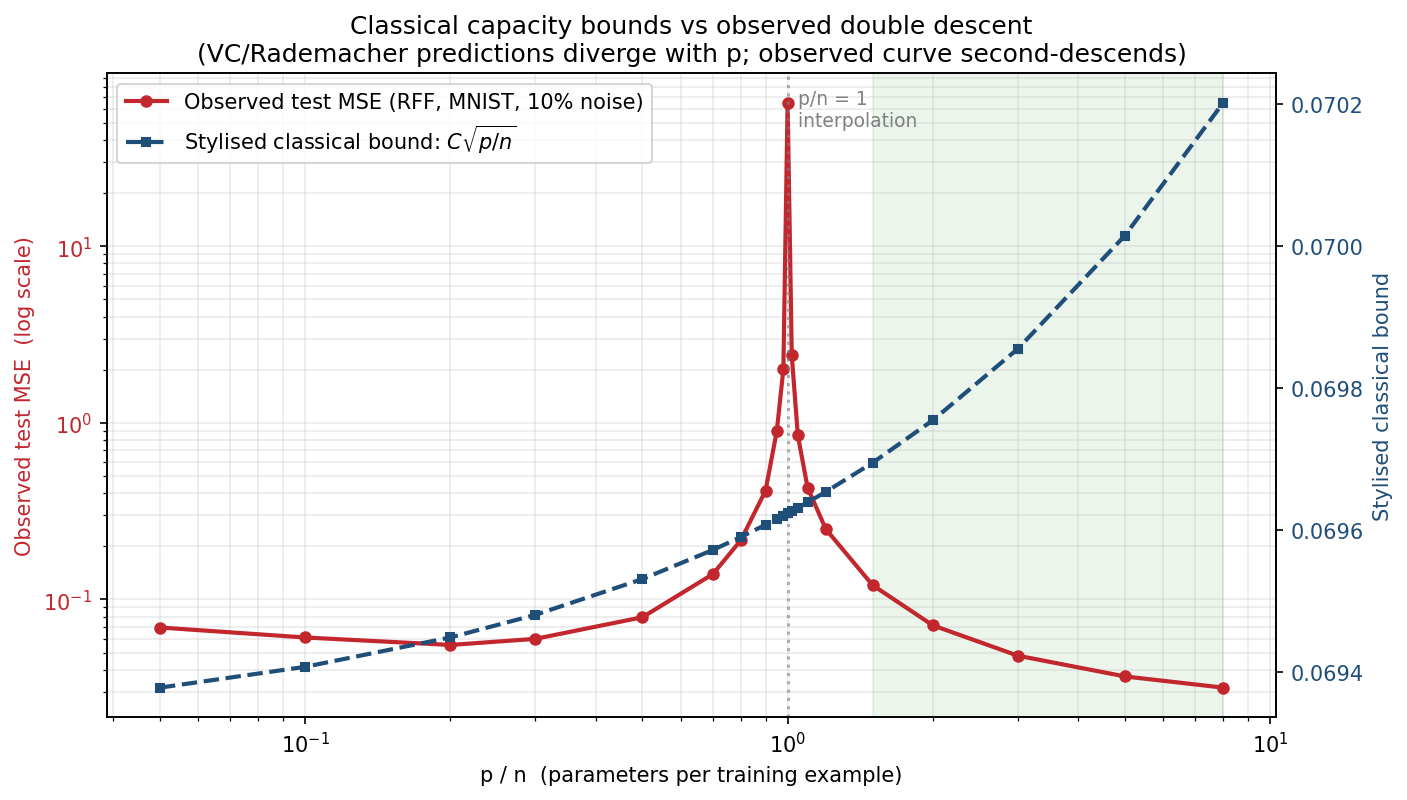
\includegraphics[width=0.55\textwidth]{figures/personD_bound_vs_observed.png}
  \caption{Classical norm-based bounds vs.\ observed test risk on the fractional-$k$ family. The bound is $\sim$$10^4 \times$ the observed value in the over-parameterised regime.}
  \label{fig:bounds}
\end{figure}

\section{Calibrated Bartlett bound vs.\ observed risk}
\label{app:bartlett}

\citet{bartlett2020benign} Theorem 1 expresses a generalisation bound through the effective rank $r_k(\Sigma)$ of the learned-feature covariance $\Sigma$, defined in \cref{eq:bartlett}. For each $k$ we evaluate $B(k)\propto \sqrt{r_k(\Sigma)/n}$, rescaled to coincide with observed risk at the smallest width to absorb the Bartlett constant, and report the vacuity ratio $B(k)/\mathcal{R}(k)$. A ratio of $1$ is tight; $\gg 1$ is loose. \cref{tab:bartlett-vacuity} reports the result on the trained fractional-$k$ ResNet.

\begin{table}[h]
  \centering
  \small
  \caption{Bartlett-style bound calibration on the trained fractional-$k$ ResNet. Effective rank climbs monotonically with $k$ ($1.14\!\to\!5.99$); the calibrated bound is essentially tight at small widths (vacuity $\approx 1$ for $k \le 0.125$) but progressively loose past the recovery onset (vacuity $\approx 1.95$ at $k\!=\!0.1875$, $3.42$ at $k\!=\!2$).}
  \label{tab:bartlett-vacuity}
  \begin{tabular}{rrrrrr}
    \toprule
    $k$ & params & $r_k(\Sigma)$ & PR & $\mathcal{R}$ (test) & vacuity $B/\mathcal{R}$ \\
    \midrule
    $0.0625$ & $823$    & $1.32$ & $1.63$  & $0.7431$ & $\mathbf{0.971}$ \\
    $0.125$  & $2{,}988$ & $1.14$ & $1.29$  & $0.6711$ & $\mathbf{1.000}$ \\
    $0.1875$ & $6{,}505$ & $2.48$ & $4.29$  & $0.5083$ & $1.948$ \\
    $0.25$   & $11{,}374$ & $2.66$ & $4.80$  & $0.4770$ & $2.147$ \\
    $0.5$    & $44{,}370$ & $3.98$ & $7.45$  & $0.4882$ & $2.567$ \\
    $1.0$    & $175{,}258$ & $5.70$ & $10.31$ & $0.4714$ & $3.184$ \\
    $2.0$    & $696{,}618$ & $5.99$ & $10.27$ & $0.4494$ & $\mathbf{3.424}$ \\
    \bottomrule
  \end{tabular}
\end{table}

This is consistent with Bartlett's theorem applying most cleanly in the linear-feature regime; trained ResNets past the recovery onset appear to leave that regime, and an unmodified Bartlett-style proxy does not deliver a tight numerical bound there. We \emph{do not} claim our work tightens the bound. The honest reading is that $r_k(\Sigma)$ is a useful \emph{diagnostic} of representation complexity --- one of five witnesses moving together through the phase transition --- but not a tight risk predictor for trained over-parameterised ResNets.

\section{Activation ablation: DD-recovery is not ReLU-specific}
\label{app:activation}

The five spectral witnesses of \cref{sec:spectral} all describe properties of the trained ResNet's representation and loss landscape; a natural follow-up is whether the recovery onset is an artefact of the ReLU nonlinearity or a property of the spectral mechanism itself. We hold everything else fixed at the recovery onset $k\!=\!0.1875$ ($n\!=\!4{,}000$, depth $3$, fractional widths $(3,6,12)$, $p\!=\!6{,}505$, $1{,}500$ epochs, two seeds) and swap only the activation function.

\begin{table}[h]
  \centering
  \small
  \caption{Test accuracy at the DD-recovery onset $k\!=\!0.1875$ across three activations. GELU recovers and \emph{beats} ReLU by $+1.7$\,pp; Tanh under-performs by roughly two points. The recovery onset survives the activation swap, so the mechanism is spectral, not ReLU-specific.}
  \label{tab:activation}
  \begin{tabular}{lrrl}
    \toprule
    Activation & Seed 42 & Seed 7 & Mean ($\Delta$ vs ReLU) \\
    \midrule
    ReLU       & $48.09\%$ & $48.28\%$ & $48.19\%$ \\
    \textbf{GELU} & $48.82\%$ & $50.94\%$ & $\mathbf{49.88\%}$ ($+1.69$\,pp) \\
    Tanh       & $47.36\%$ & $44.94\%$ & $46.15\%$ ($-2.04$\,pp) \\
    \bottomrule
  \end{tabular}
\end{table}

The within-activation seed spread ($\le 2.1$ pp) is comparable to the cross-activation gap, so the ranking is robust but the precise margin would tighten with a larger seed cohort. The crucial qualitative result is that the recovery onset survives the activation swap. We did not measure whether GELU shifts the onset $k$ itself; a $k$-sweep $\times$ activation grid is the obvious next experiment and is listed under \cref{sec:discussion} future work.

\section{Lecture mapping}
\label{app:lectures}

Every experiment in this paper is anchored to at least one EECS 6699 (Mathematics of Deep Learning, Spring 2026) lecture concept. \cref{tab:lectures} makes the mapping explicit and doubles as a reading guide.

\begin{table}[h]
  \centering
  \small
  \caption{Lecture mapping for every numbered experiment. Lecture numbers refer to L1--L12 as delivered; the same theory anchors recur across the kernel and NN halves of the pipeline.}
  \label{tab:lectures}
  \resizebox{\linewidth}{!}{%
  \begin{tabular}{lll}
    \toprule
    Section / experiment & Primary lecture concept & Lectures \\
    \midrule
    \cref{sec:rff} RFF model-wise (Exp.~1) & Variance explosion at interpolation threshold & L1--L2, L9 \\
    \cref{sec:rff} RFF sample-wise (Exp.~2) & Effective dimension scales with $n$ & L9--L10 \\
    \cref{sec:rff} bias-variance & Risk decomposition & L1--L2 \\
    \cref{sec:rff} ridge sweep (Person A) & Ridge regularisation smooths peak & L10 \\
    \cref{sec:rff} noise sweep (Person B) & Noise as a stress test for interpolation & L1--L2, L9 \\
    \cref{sec:nn} fractional-$k$ DD-Recovery & NN expressivity vs.\ sample size; Barron approximation & L2--L3, L5--L6 \\
    \cref{sec:samplewise} sample-wise NN DD & Peak shifts with $n$ on NN & L9--L10 \\
    \cref{sec:spectral} W1, W2: penultimate spectrum & Last-layer NTK; Bartlett benign overfitting & L7--L8, L10 \\
    \cref{sec:spectral} W3: full empirical NTK & NTK / lazy training & L7--L8 \\
    \cref{sec:spectral} W5: Hessian top eig & Optimisation landscape; SAM flatness & L5--L6 \\
    \cref{sec:audit} metric audit & Evaluation protocol; generalisation measurement & L9--L12 \\
    \cref{app:optimizer} Adam vs.\ SGD (Person C) & Implicit-bias comparison & L5--L6 \\
    \cref{app:optimizer} Person D bounds & Norm-/margin-based generalisation bounds & L9--L12 \\
    \cref{app:bartlett} Bartlett bound calibration & Effective rank vs.\ observed risk & L9--L10 \\
    \cref{app:ablations} depth ablation & Approximation theory and depth & L2--L3 \\
    \cref{app:activation} activation ablation & Implicit regularisation by activation choice & L5--L6 \\
    \bottomrule
  \end{tabular}}
\end{table}

\section{Depth ablation: DD-recovery is depth-robust}
\label{app:ablations}

To address how \emph{depth} impacts NN performance on this task, we extend the fractional-$k$ family to a configurable-depth variant in which the number of stages is a parameter and widths follow the same doubling pattern $(c_1,c_2,\ldots) = (\max(1, 16k), 32k, 64k,\ldots)$. At fixed $k\!=\!0.5$ (over-parameterised; otherwise identical to \cref{sec:nn}), two seeds, we compare depths $\in\{2, 3, 4\}$.

\begin{table}[h]
  \centering
  \small
  \caption{Best test accuracy at $k\!=\!0.5$ across three depths. The DD-recovery shape is preserved at all three depths (best test accuracy stays in the $47\!-\!53\%$ band, well above the $24.9\%$ under-fit baseline at $k\!=\!0.0625$); lean depth wins on noisy data.}
  \label{tab:depth-ablation}
  \begin{tabular}{lllr}
    \toprule
    Depth & Stage widths & Params & Best test acc (mean $\pm$ std, two seeds) \\
    \midrule
    $2$ & $(8, 16)$ & $11{,}122$ & $\mathbf{52.14\% \pm 1.54}$ \\
    $3$ & $(8, 16, 32)$ & $44{,}370$ & $51.18\%$ (1 seed; \cref{sec:nn} baseline) \\
    $4$ & $(8, 16, 32, 64)$ & $176{,}402$ & $47.77\% \pm 0.88$ \\
    \bottomrule
  \end{tabular}
\end{table}

The recovery shape is preserved at all three depths. \emph{Lean depth wins on noisy data}: depth 2 outperforms depths 3 and 4 on average; depth 4 exhibits classic over-parameterised label memorisation with best test accuracy peaking at epoch $\sim 200$ ($\sim 46\!-\!48\%$) and then declining as training continues to memorise noise. Smaller depth at fixed $k$ acts as a regulariser, mirroring the early-stopping benefit observed for over-parameterised $k$ (\cref{app:epochwise}). We test depth 2--4 at a single $k$; a full $k\!\times\!\text{depth}$ grid would be required to track whether the recovery onset $k^\star$ shifts with depth, and is left as future work.

\section{Epoch-wise dynamics on fractional-$k$}
\label{app:epochwise}

We additionally run an epoch-wise protocol at three focal widths $k\in\{0.125, 0.1875, 0.5\}$, holding aside $10\%$ of the training subset as validation. \cref{fig:epochwise} plots test accuracy vs.\ epoch and the gap $\Delta = \mathrm{best\_test} - \mathrm{final\_test}$ on a per-seed basis. The over-parameterised side ($k\!=\!0.5$) shows positive $\Delta$ of $1.5$--$2.7$ pp with validation-best epochs at $800$--$1{,}175$ --- the classic late-training overfitting under label noise. Near the threshold ($k\!=\!0.1875$) and on the under-fit side ($k\!=\!0.125$), $\Delta$ is slightly negative ($-0.2$ to $-1.1$ pp): test accuracy at epoch $2{,}000$ exceeds the validation-argmax checkpoint, so validation-based early stopping does not improve test accuracy. The metric audit of \cref{sec:audit} and this epoch-wise picture describe complementary slices of the same training instability.

\begin{figure}[h]
  \centering
  \begin{subfigure}{0.49\textwidth}
    
\includegraphics[width=\linewidth]{figures/fractionalk_epochwise.png}
    \caption{Epoch-wise dynamics: test accuracy vs.\ epoch.}
  \end{subfigure}\hfill
  \begin{subfigure}{0.49\textwidth}
    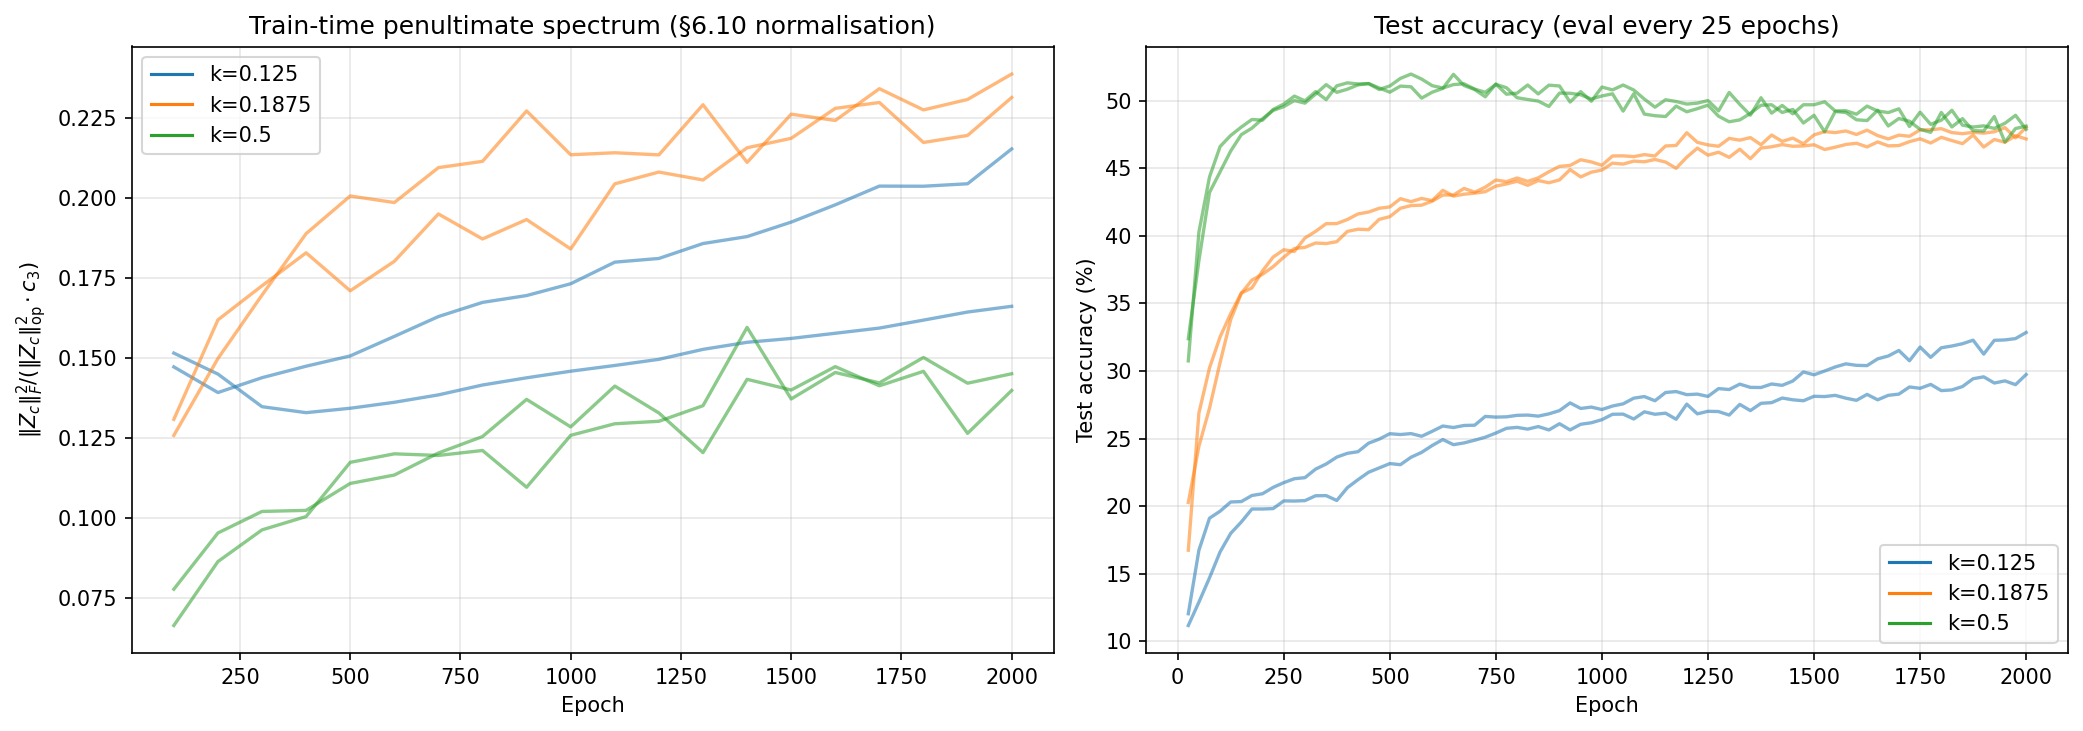
\includegraphics[width=\linewidth]{figures/fractionalk_epochwise_spectral.png}
    \caption{Train-time penultimate stable rank vs.\ epoch.}
  \end{subfigure}
  \caption{Epoch-wise dynamics on the fractional-$k$ family at three focal widths.}
  \label{fig:epochwise}
\end{figure}

\section{Reproduction details}
\label{app:repro}

\paragraph{Code.} Repository URL withheld for review; will be released on publication. The directory layout in the supplementary material mirrors the entries below. Entry points: \texttt{src/experiments/comprehensive\_dd.py} for RFF Exps 1--2, \texttt{src/experiments/exp\_dd\_recovery.py} for the fractional-$k$ campaign, \texttt{src/experiments/exp\_samplewise\_nn.py} for \cref{sec:samplewise}, \texttt{src/experiments/personA\_ridge\_sweep.py} / \texttt{personB\_noise\_sweep.py} / \texttt{personC\_optimizer\_compare.py} / \texttt{personD\_bounds\_figure.py} for \cref{sec:rff} and \cref{app:optimizer}.

\paragraph{Hardware.} All training runs use a single A100 (80\,GB) or RTX-5090 (32\,GB). RFF experiments run on CPU in $<\!90$ seconds. The DD-Recovery campaign is $\sim$$10$ GPU-hours per seed; the full $9$-point $k$ grid with two seeds is $\sim$$20$ GPU-hours. Sample-wise sweep adds $\sim$$8$ GPU-hours.

\paragraph{Random seeds.} RFF experiments use $5$ seeds $\{42, 123, 456, 789, 1024\}$; NN experiments use $2$ seeds $\{42, 7\}$; the noise-sweep multi-seed audit (Person B) uses $3$ seeds $\{42, 7, 123\}$.

\end{document}
